% \section*{Mô hình sinh cử chỉ OHGesture}

% \section*{3 Phương Pháp Của Chúng Tôi}
% Diffusion là mô hình đằng sau các thành công của  Stable Diffusion, Midjourney và DALL-E trong việc tạo ra các tấm ảnh siêu thực.


%. Biếm tiềm ẩm ở đây là cử chỉ và điều kiện là cảm xúc. 
%Kiến trúc của OHGesture được trình bày như hình \autoref{fig:diffusion_forward}.
\pagebreak

\section{Mô hình của đề xuất OHGesture}
\label{sec:ohgesture}

%\begin{figure}
%	\centering
%	\includegraphics[width=\linewidth]{images/diffusion_forward}
%	\caption{Minh hoạ quá trình khử nhiễu (denoising) cử chỉ}
%	\label{fig:diffusion_forward}
%\end{figure}

%\begin{figure*}
%	\centering
%	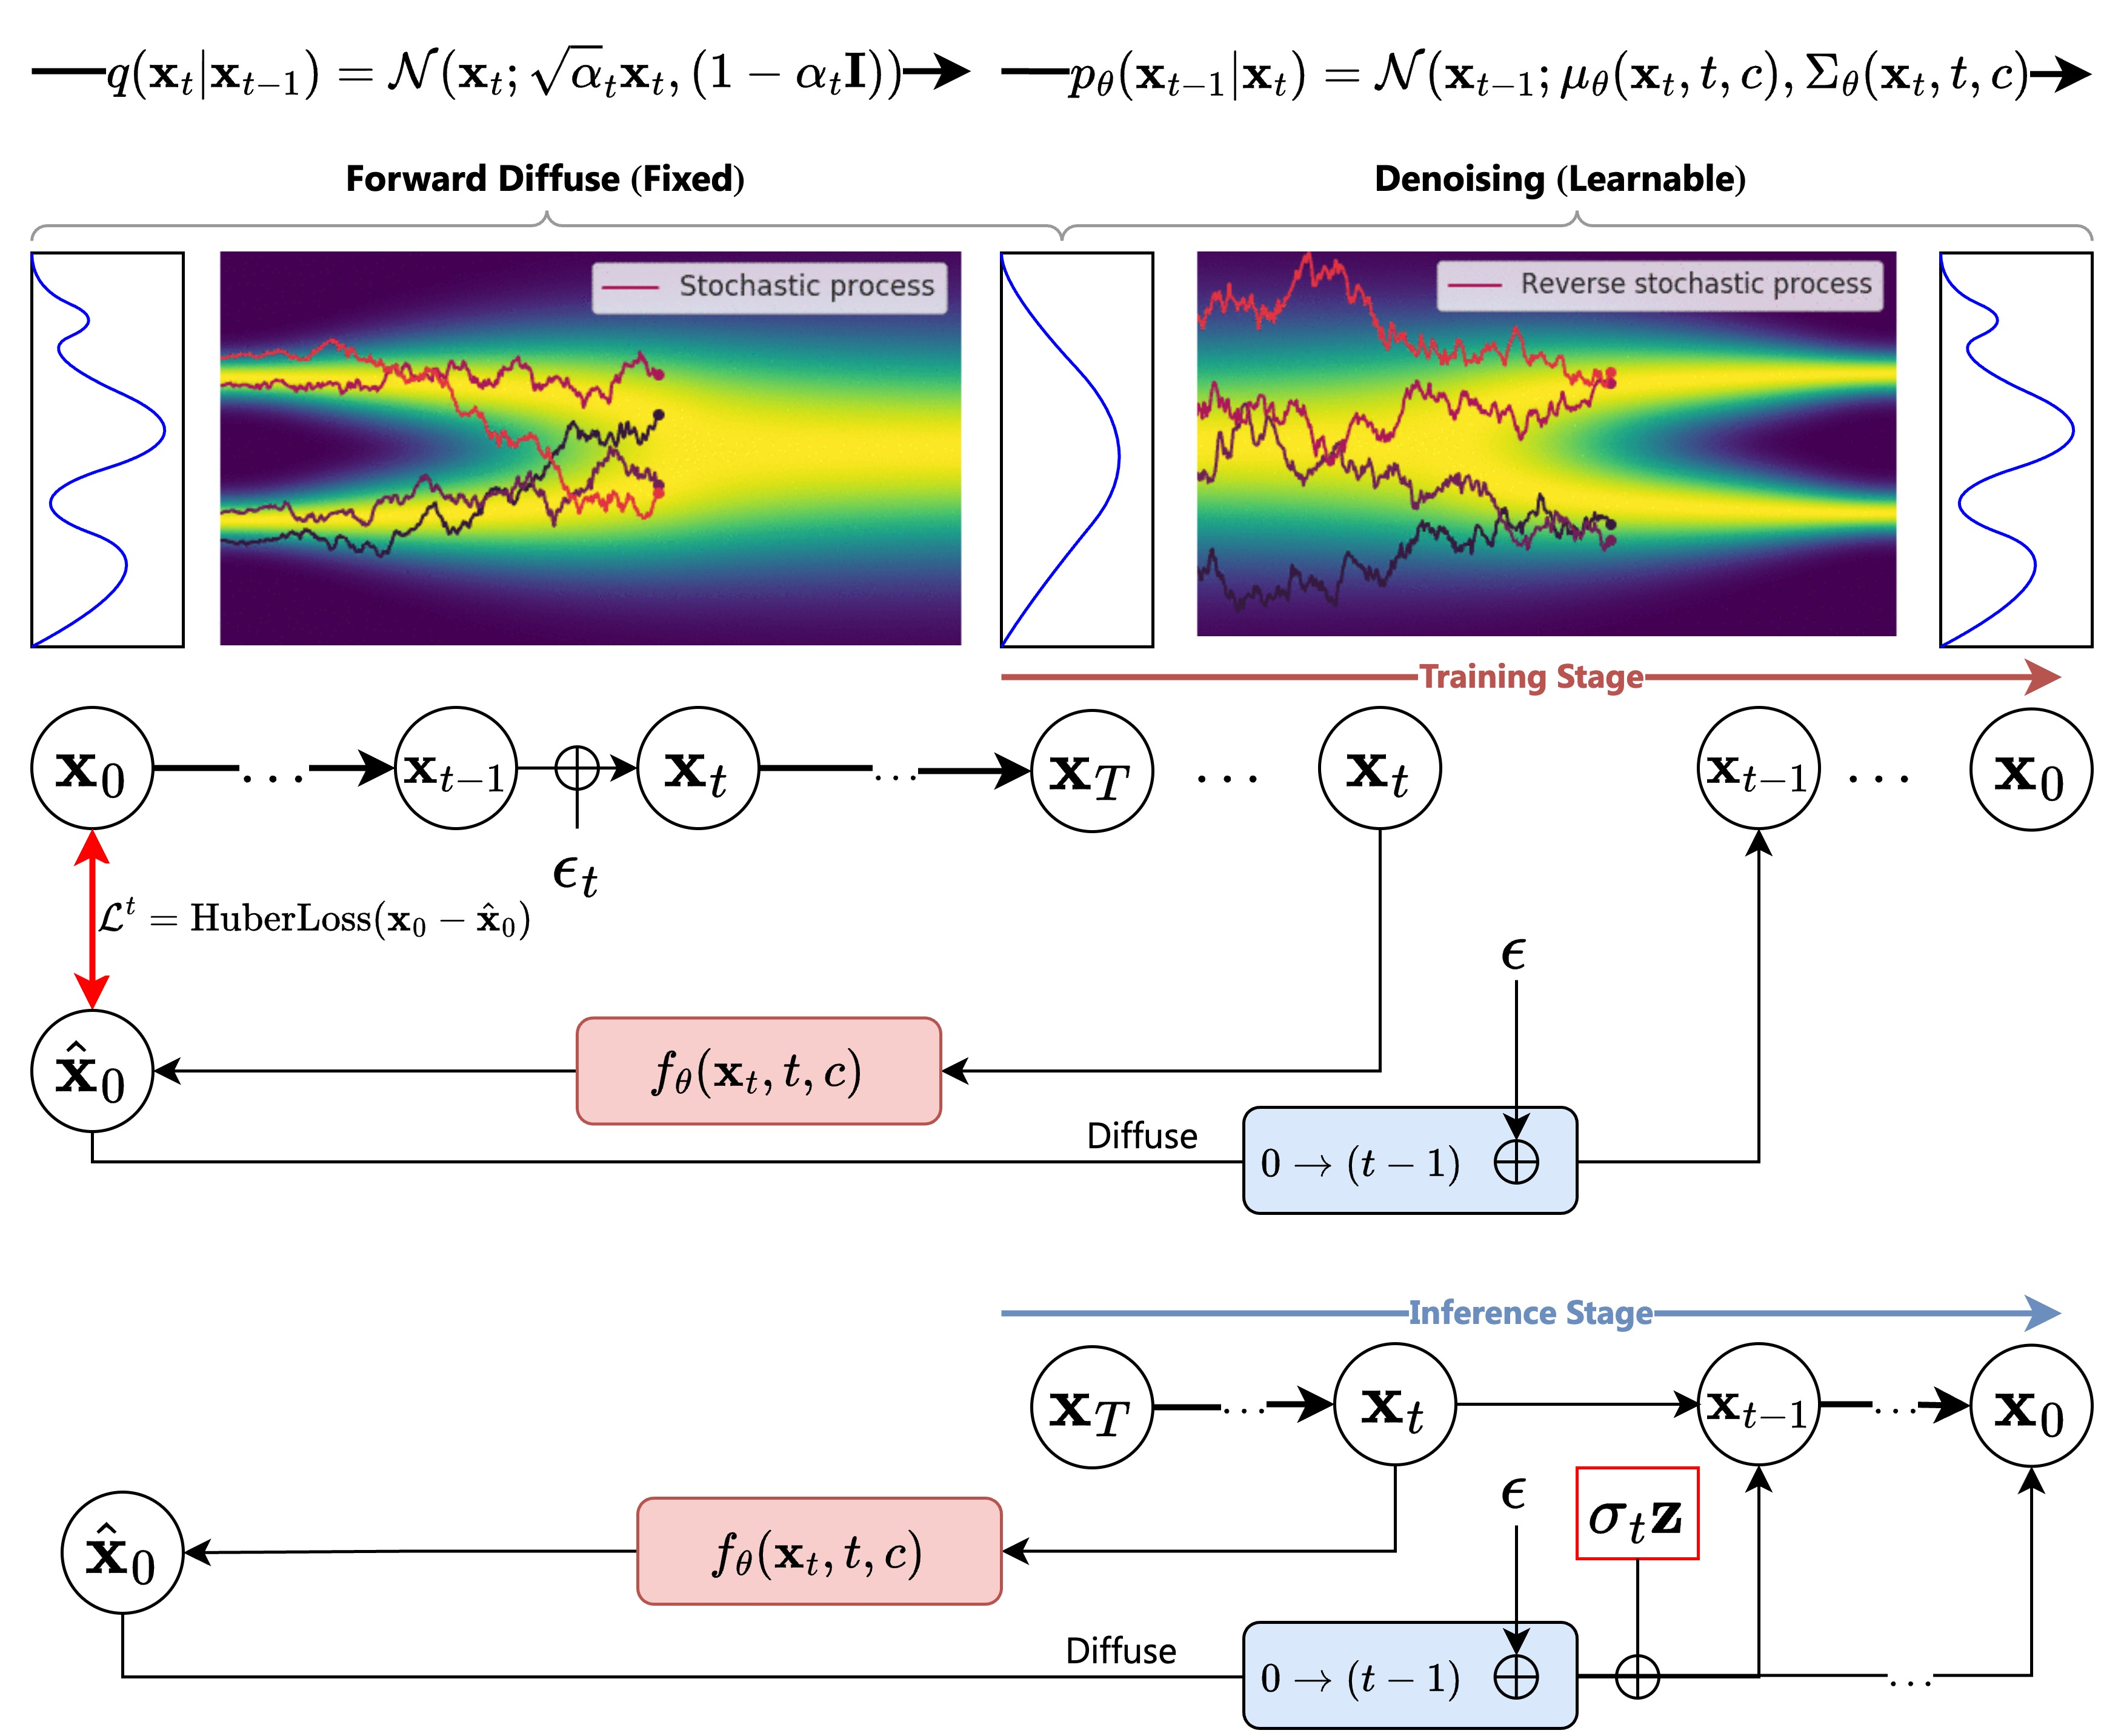
\includegraphics[width=0.8\linewidth]{TrainingAndSampling}
%	\caption{Quá trình Huấn luyện và lấy mẫu trong OHGesture}
%%	\label{fig:TrainingAndSampling}
%\end{figure*}

\begin{figure}[H]
	\centering
	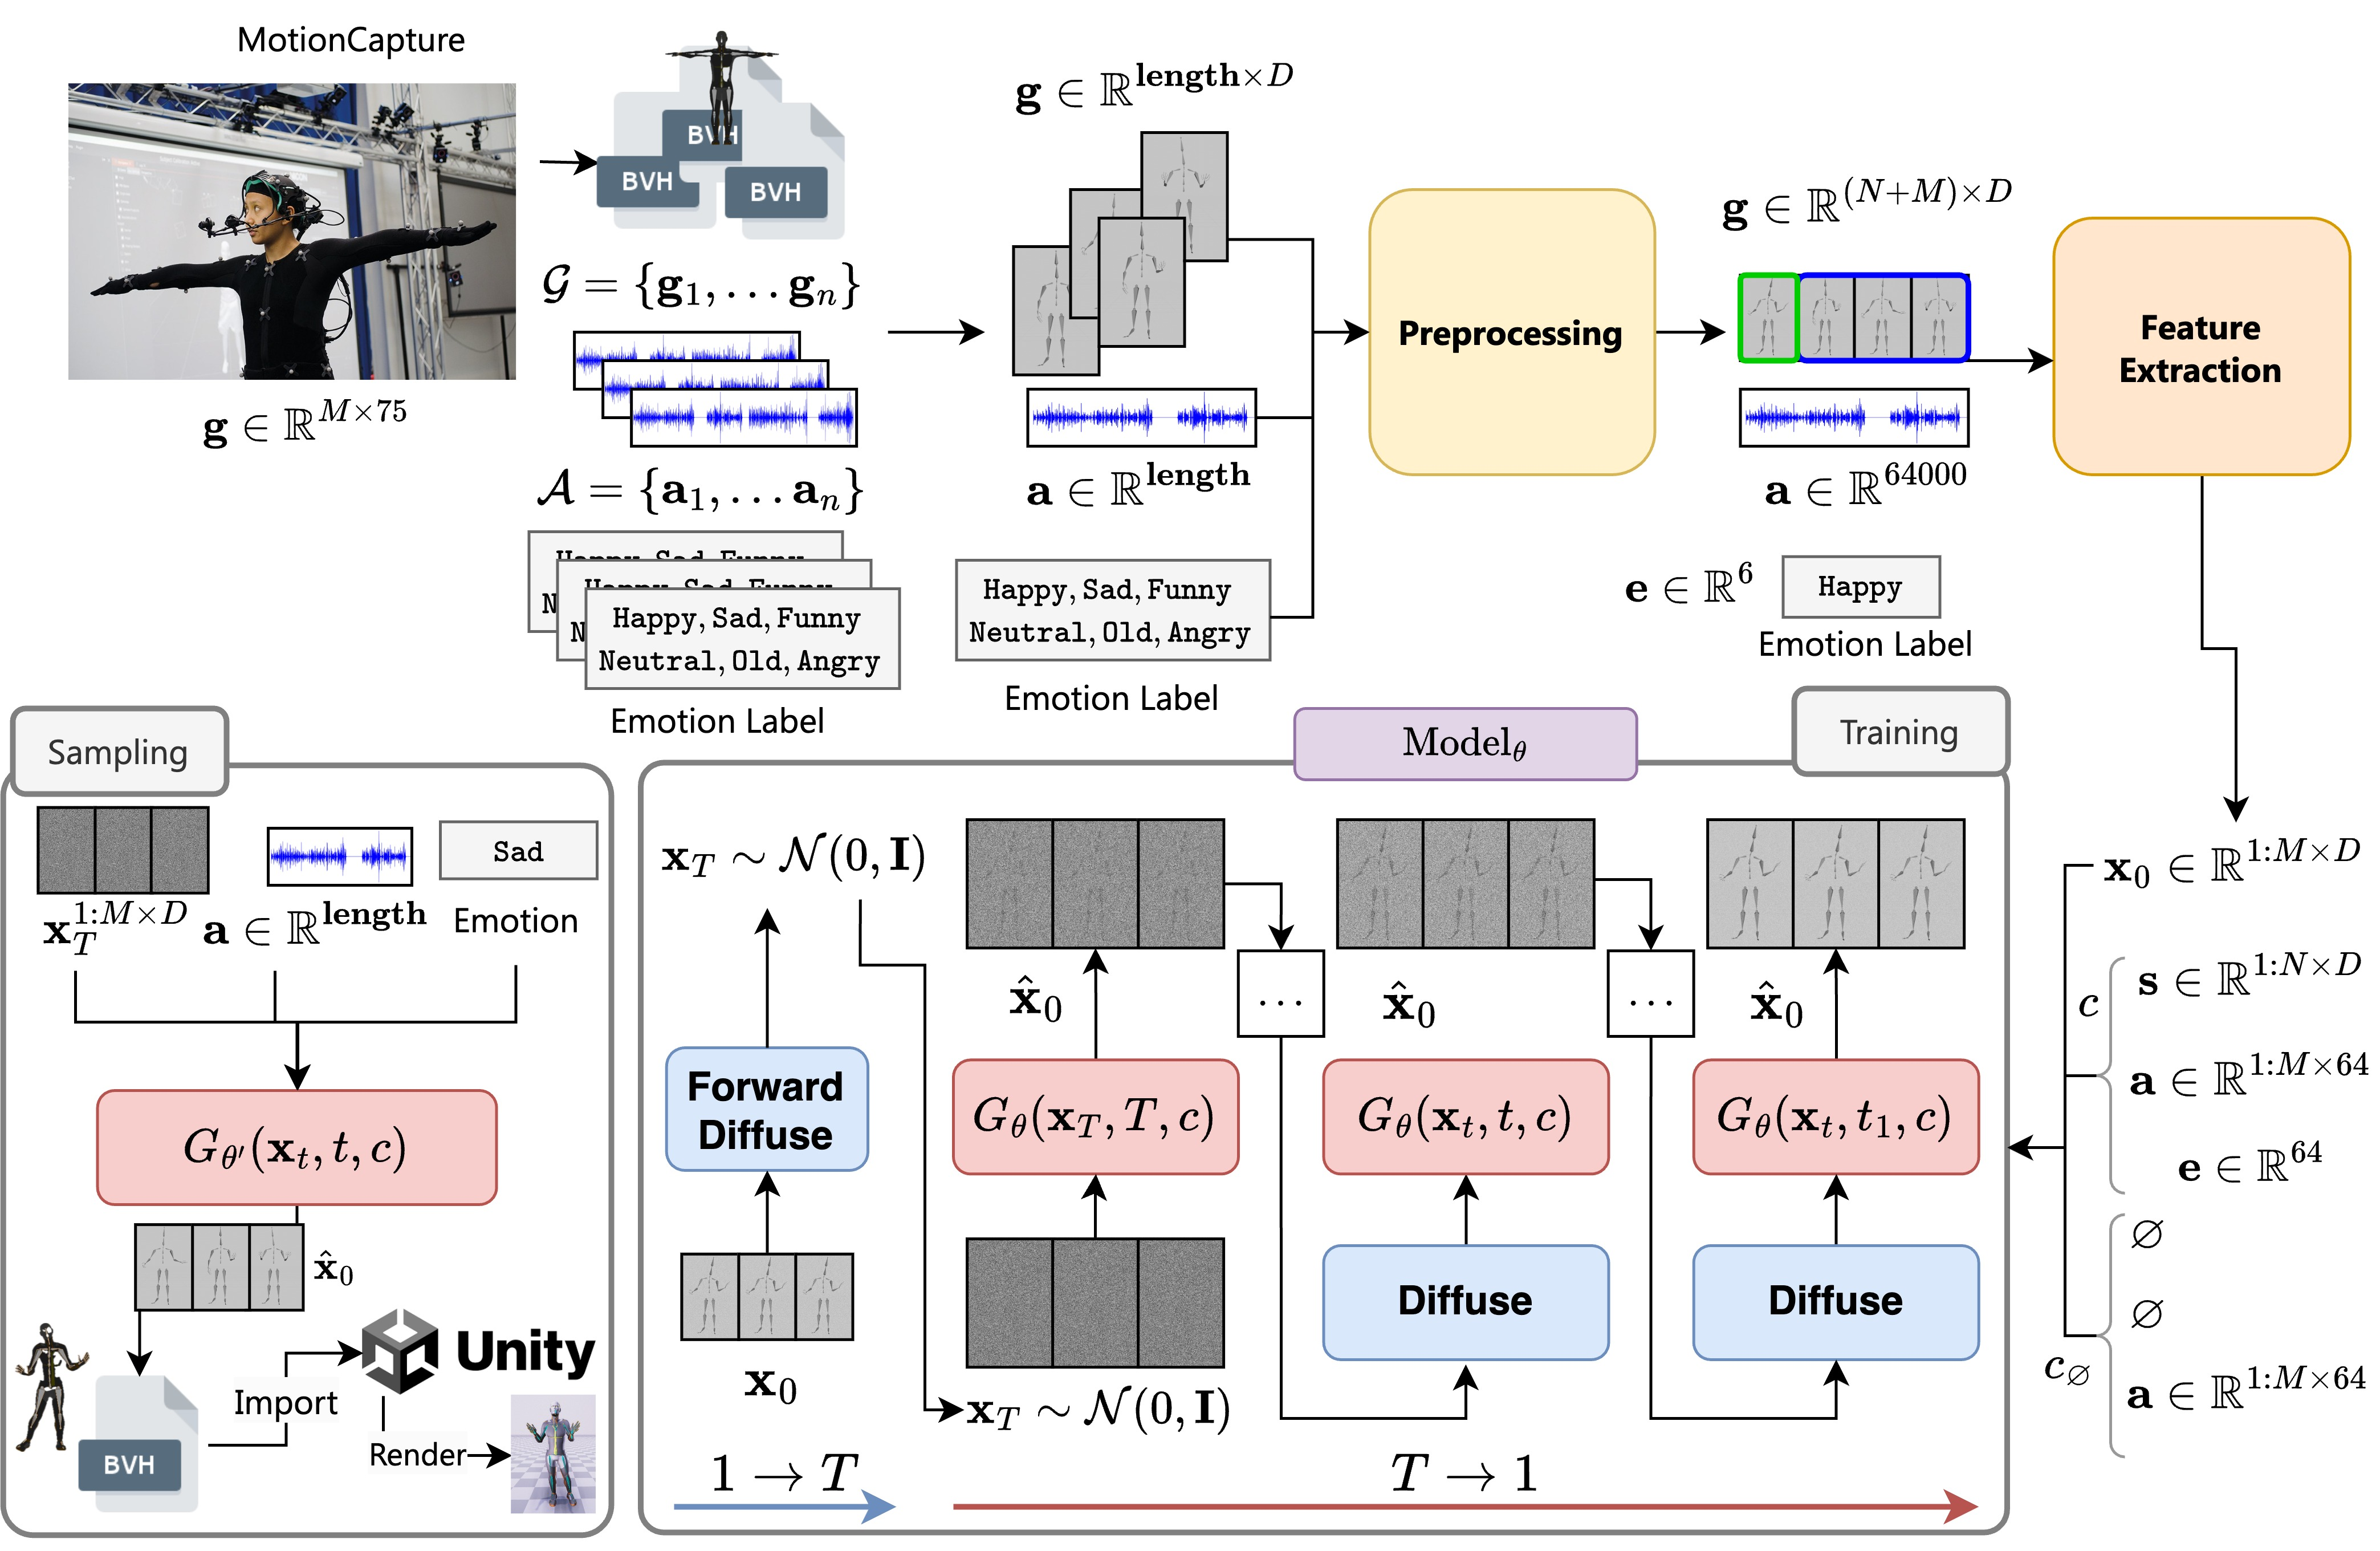
\includegraphics[width=\linewidth]{AllStage}
	\caption{Quá trình Huấn luyện và lấy mẫu trong OHGesture}
	\label{fig:TrainingAndSampling}
\end{figure}

Mô hình đề xuất \textbf{OHGesture} của chúng tôi được dựa trên mô hình \textbf{DiffuseStyleGesture} \cite{yang2023diffusestylegesture} áp dụng mô hình Diffusion \cite{ho2020denoising} có điều kiện \cite{ho2022classifier} (Classifier-Free Diffusion Guidance) để điều khiển các đặc trưng trong quá trình khử nhiễu. 
Không giống như trong mô hình DiffuseStyleGesture, chúng tôi sử dụng thêm điều kiện văn bản được nhúng bằng mô hình Pretrain FastText  \cite{bojanowski2017enriching}.

Những điểm giống và khác của việc áp dụng mô hình Diffusion cho bài toán sinh cử chỉ so với mô hình Diffusion trong bài toán sinh ảnh:

\vspace{10pt}

\textbf{Điểm giống}
\begin{itemize}
	\item Chúng tôi sử dụng mô hình Diffusion \cite{yang2023diffusestylegesture} trên cử chỉ $\bx^{1:M \times D}$,  với $M$ frame theo thời gian, $D=1141$ là các điểm toạ độ chuyển động của mỗi khung hình (tương tự width và height trong ảnh).
	\item Classifier-Free Diffusion Guidance với $\bx_0$ objective.
	\item Latent vector có số chiều là $256$.
\end{itemize}

\textbf{Điểm khác}

\begin{itemize}
	\item Sinh cử chỉ có điều kiện:
	\begin{itemize}
		\item Điều kiện cảm xúc: $c = \big[ \mathbf{s}, \mathbf{e}, \mathbf{a}, \mathbf{v} \big]$ và $c_{\varnothing} = \big[ \varnothing, \varnothing, \mathbf{a}, \mathbf{v}\big]$.
		\item Nội suy trạng thái giữa hai cảm xúc $\mathbf{e}_1, \mathbf{e}_2$, sử dụng điều kiện: $c = \big[ \mathbf{s}, \mathbf{e}_1, \mathbf{a}, \mathbf{v} \big]$ và $c_{\varnothing} = \big[ \mathbf{s}, \mathbf{e}_2, \mathbf{a}, \mathbf{v} \big]$.
	\end{itemize}
	\item Self-Attention: Mối liên hệ giữa các cảm xúc, cử chỉ khởi tạo và từng frame (tương tự DALL-E 2 - mối liên hệ giữa văn bản và ảnh).
	\item Concat âm thanh và văn bản (Giống ControlNet - Pixel-wise Condition)
	%			\item Học mối liên hệ giữa điều kiện và các frame bằng Local-Cross Attention
\end{itemize}

Trong đó $\bx_0$ là chuỗi $M$ khung hình cử chỉ $\mathbf{x} \in \mathbb{R}^{1:M \times D}$ ($D = 1141$), với điều kiện $c = [\mathbf{s}, \mathbf{e}, \mathbf{a}, \mathbf{v}]$ bao gồm cử chỉ khởi tạo (seed gesture) $\mathbf{s}$,  cảm xúc (emotion) $\mathbf{e}$, chuỗi âm thanh (audio) $\mathbf{a}$ tương ứng cử chỉ, và văn bản  $\mathbf{v}$.
%} \in \mathbb{R}^{M \times 300} 
%, chuỗi âm thanh thô $64000$ là $4$ giây với mỗi giây được đọc với sample rate là $16000$.

%Với đầu vào bao gồm cử chỉ khởi tạo $x_{\text{seed}}$, âm thanh $a$ và văn bản $t$.
% với biến tiềm ẩn   (diffusion latent variable)
Tương tự mô hình diffusion cơ bản bao gồm hai quá trình: quá trình tạo nhiễu (diffusion) $q$ và quá trình khử nhiễu (denoising process) $p_{\theta}$ với trọng số $\theta$. Quá trình Training và Sampling của mô hình đề xuất \textbf{OHGesture} được minh hoạ ở hình \ref{fig:TrainingAndSampling}.

\subsection{Quá trình trích xuất đặc trưng}

Dữ liệu để học của chúng tôi được lấy từ tập dữ liệu ZeroEGGS \cite{ghorbani2022zeroeggszeroshotexamplebasedgesture}. Bao gồm âm thanh, cử chỉ khởi tạo, cảm xúc và văn bản.
%Tương tự mô hình DiffuseStyleGesture \cite{yang2022DiffuseStyleGestureplus} chúng tôi cũng sử dụng đầu vào bao gồm âm thanh, cử chỉ và cảm xúc
%ngoài ra chúng tôi sử dụng thêm dữ liệu văn bản.
\begin{figure}[H]
	\centering
	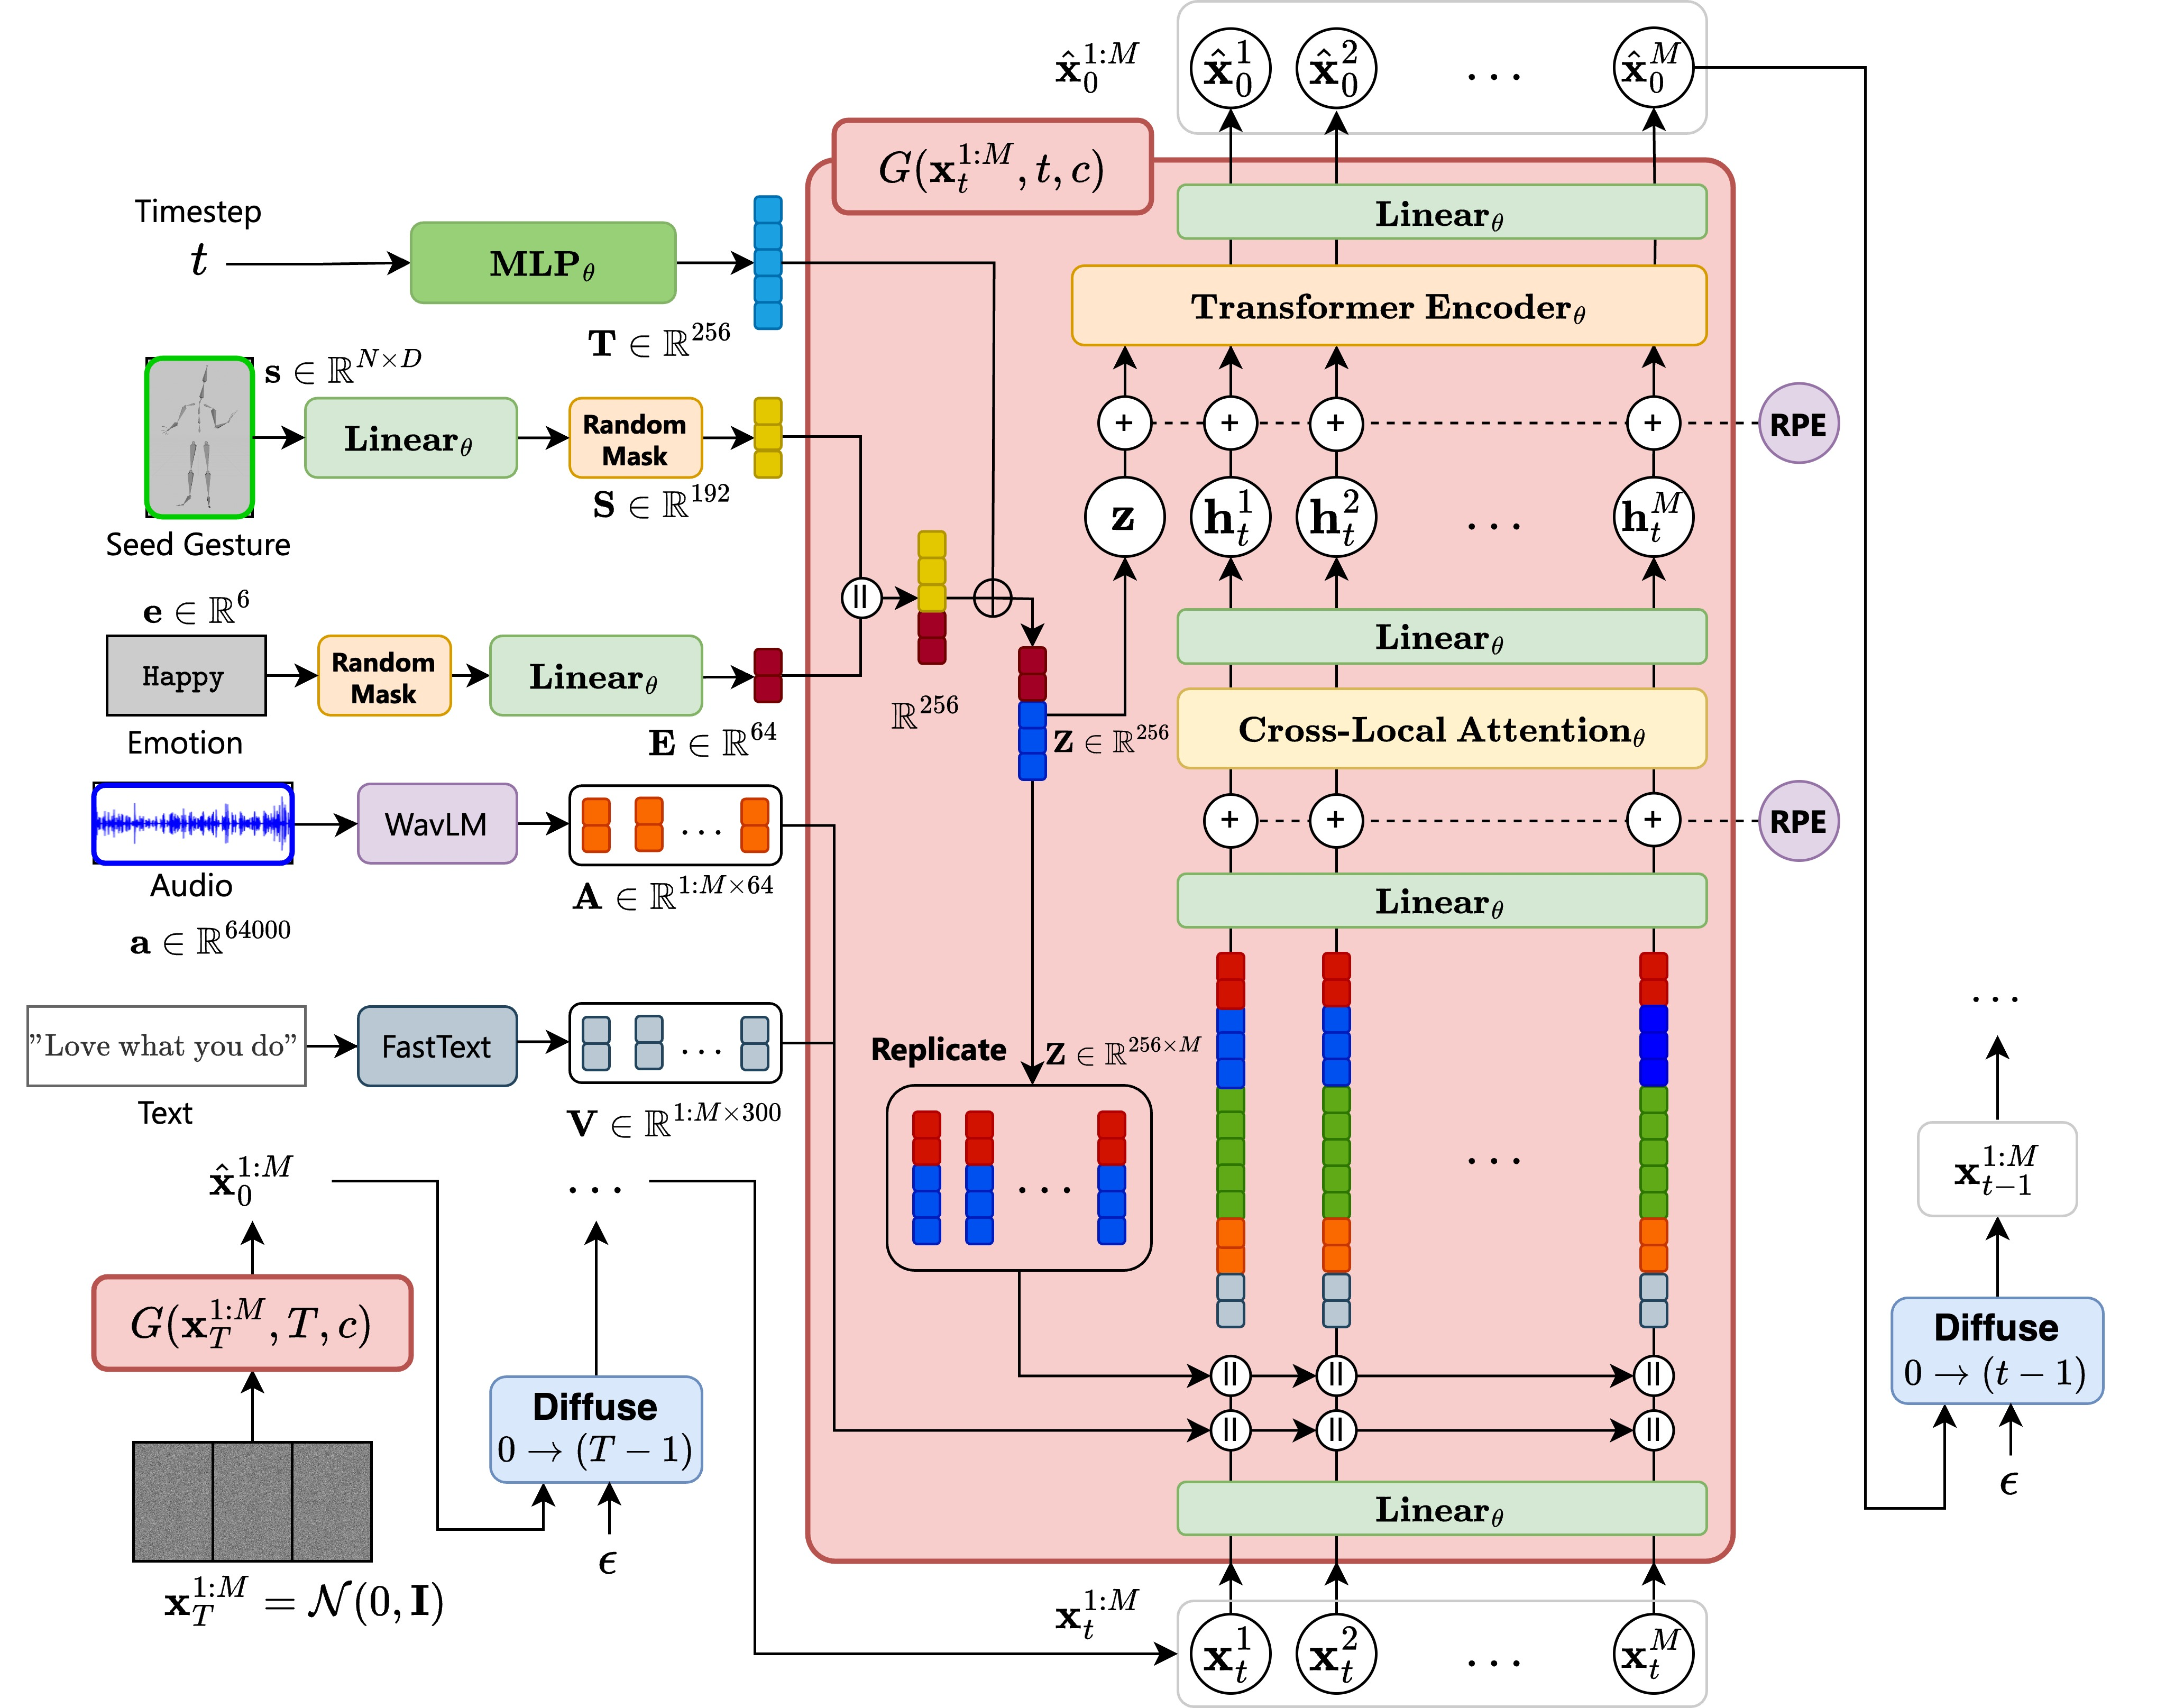
\includegraphics[width=\textwidth]{OHGesture}
	\caption{Mô hình trong OHGesture}
	\label{fig:OHGesture}
\end{figure}
\vspace{-10pt}

\begin{itemize}
	\item \textbf{Bước thời gian $\mathbf{T} \in \mathbb{R}^{256}$ }: Bước thời gian ở mỗi quá trình $t \in [0, T]$, mục tiêu của mô hình là để với bước thời gian $t$ bất kỳ, mô hình có thể tổng quát hoá quá trình khử nhiễu, và có thể học được việc với từng bước $t$ thì giá trị sẽ thay đổi thế nào đối với kết quả dự đoán $\bx_0$. Giá trị timestep $t$ được khởi tạo bằng việc mã hoá nhúng vị trí (Position Embedding) bằng hàm sinusoidal $\text{PE}(t) = \left[ \sin{\left(\frac{t}{10000^{2i / d}}\right)}, \cos{\left(\frac{t}{10000^{2i / d}}\right)} \right]$, sau đó được đưa vào một MLP (Multilayer perceptron) để biến đổi thành vector $\mathbf{T}  \in \mathbb{R}^{256}$.
	
	\item \textbf{Cử chỉ khởi tạo $\mathbf{S} \in \mathbb{R}^{192}$}: Cử chỉ khởi tạo (seed gesture) $\mathbf{s} \in \mathbb{R}^{1:N \times D}$ có được từ cử chỉ ground truth $
	\mathbf{g} \in \mathbb{R}^{(N+M) \times D}$, với mỗi frame là dữ liệu bao gồm $75$ khớp xương, được xử lý theo công thức \ref{eq:gesturevector} để được vector $1141$ chiều, trình bày ở công thức \ref{eq:gesturevector}. Chúng tôi cắt $N = 8$ frame đầu để làm cử chỉ khởi tạo $\mathbf{s}$ và $M = 80$ (4 giây với $20fps$) frame tiếp theo là nhãn để thực hiện quá trình khử nhiễu $\mathbf{x}^{1:M}$. Vector $\mathbf{s}$ đi qua một lớp tuyến tính để được vector $\mathbf{S} \in \mathbb{R}^{192}$, vector $\mathbf{S}$ sau đó được Random Mask trong quá trình huấn luyện để bỏ trong trường hợp nếu một trong $N$ bị thiếu thì sẽ ảnh hưởng như thế nào đến cử chỉ dự đoán.
%	Quá trình này được minh hoạ ở hình \ref{fig:GestureSeries}.
	
%	\item\textbf{Âm thanh}: Âm thanh sẽ được dùng làm đặc trưng để sinh cử chỉ, Chúng tôi sử dụng các mô hình Pretrain có sẵn như WavLM \cite{chen2022wavlm} để trích xuất đặc trưng âm thanh. 
%	Chúng tôi kết hợp thêm các đặc trưng về MFCC, Mel-Spectrum, Pitch, Enery và Onsets \cite{bello2005tutorial}
  \item \textbf{Âm thanh $\mathbf{A} \in \mathbb{R}^{1:M \times 64}$}: Tất cả dữ liệu âm thanh được giảm số sample rate (down sampled) xuống $16 \mathrm{kHz}$, và âm thanh sẽ được lấy tương ứng với cử chỉ là 4s để được vector $\mathbf{a} \in \mathbb{R}^{64000}$, chúng tôi sử dụng mô hình pre-train của WavLM Large \cite{Chen_2022} nhúng waveform thô vào  để được vector tiềm ẩn. Sau đó sử dụng nội suy tuyến tính (interpolation) để căn chỉnh đặc trưng của vector tiềm ẩn trong WavLM theo chiều thời gian thành $20fps$, sau đó sử dụng một lớp tuyến tính để giảm kích thước của đặc trưng xuống còn vector đặc trưng với $64$ để tạo thành ma trận cuối cùng $\mathbf{A} \in \mathbb{R}^{M \times 64}$.
		
	\item \textbf{Cảm xúc $\mathbf{E} \in \mathbb{R}^{64}$}: Cảm xúc (emotion) $\mathbf{e} \in \mathbb{R}^{6}$ bao gồm 6 cảm xúc khác nhau được biểu diễn thành một vector theo phương pháp one-hot encoding, sau đó chúng tôi đưa qua một vector tuyến tính để được vector đặc trưng $\mathbf{E} \in \mathbb{R}^{64}$. Mục tiêu là để có thể concat được với vector khởi tạo $\mathbf{S} \in \mathbb{R}^{192} $ để tạo thành vector tiềm ẩn $256$ chiều.
	
	
%	\item \textbf{Cử chỉ nhiễu $\mathbf{x}_{T} \in \mathbb{R}^{M \times D}$} (Noisy gesture): khi huấn luyện, $\mathbf{x}_{t}$ là cử chỉ nhiễu có cùng kích thước như cử chỉ gốc $\mathbf{x}_{0}$ sẽ được sinh ngẫu nhiên từ phân phối chuẩn $\mathcal{N}(0, \mathbf{I})$. Khi sinh ngẫu nhiên, cử chỉ nhiễu ban đầu $\mathbf{x}_{T}$ được lấy mẫu từ phân phối chuẩn chuẩn và các $\mathbf{x}_{t}, t<T$ khác là kết quả của bước làm nhiễu trước đó. Sau đó, kích thước được điều chỉnh thành 256  bằng lớp biến đổi tuyến tính (linear layer).
	\item \textbf{Văn bản $\mathbf{V} \in \mathbb{R}^{1:M \times 300}$}: Văn bản là đoạn văn bản được dịch tương ứng với âm thanh, được đưa vào FastText \cite{bojanowski2017enriching} để thu được một vector có số chiều là 300. Sau đó, được replicate để căn chỉnh tương ứng với $M$ khung hình để được vector đặc trưng $\mathbf{V}$ như hình \ref{fig:OHGesture}.
\end{itemize}

%\item Bước làm nhiễu: Trong quá trình huấn luyện, bước làm nhiễu $t$ được lấy mẫu từ phân phối chuẩn của $\{1,2, \ldots, T\}$, với mã hóa vị trí (position encoding) giống như mô hình Transformer \cite{vaswani2017attention}, sau đó được ánh xạ vào không gian $\mathbf{T}$ có kích thước 256 bằng một mạng perceptron nhiều lớp (MLP).
%
%
%
%\item Cảm xúc: Các cảm xúc của cử chỉ được biểu diễn dưới dạng vectơ one-hot encoding, tức thành vector toàn bộ là số $0$ và vị trí có cảm xúc tương ứng có vị trí là $1$, vector one-hot encoding được ánh xạ vào không gian có kích thước 64 $\mathbf{S}$ thông qua một lớp tuyến tính.
%
%\item Cử chỉ khởi tạo: Cử chỉ khởi tạo giúp tạo ra sự chuyển tiếp mượt mà giữa các lần sinh liên tiếp \cite{yoon2020speech}. Cử chỉ khởi được cắt ngắn xuống $g \in$ $\mathbb{R}^{(8+N) \times 1141}$. Trong quá trình training, $8$ frame đầu tiên của cử chỉ $g$ được sử dụng làm cử chỉ khởi tạo $d$ và $N$ frame còn lại được sử dụng làm cử chỉ thật $x_{0}$ để tính hàm loss $\mathcal{L}$. Sau đó, chúng tôi ánh xạ các đặc trưng của cử chỉ khởi tạo $d$ vào không gian $\mathbf{D}$ có kích thước $192$ chiều bằng một lớp tuyến tính. 
%Kết quả cử chỉ được sinh ra trong $4$ giây, và vì cử chỉ sinh ra được chạy ở $20 \mathrm{fps}$ (tương đương 20 khung hình mỗi giây) nên kích thước $N=80$.

%\section{Mô hình diffusion cho bài toán sinh cử chỉ}
%\vspace{-20pt}
%\begin{figure}
%	\centering
%	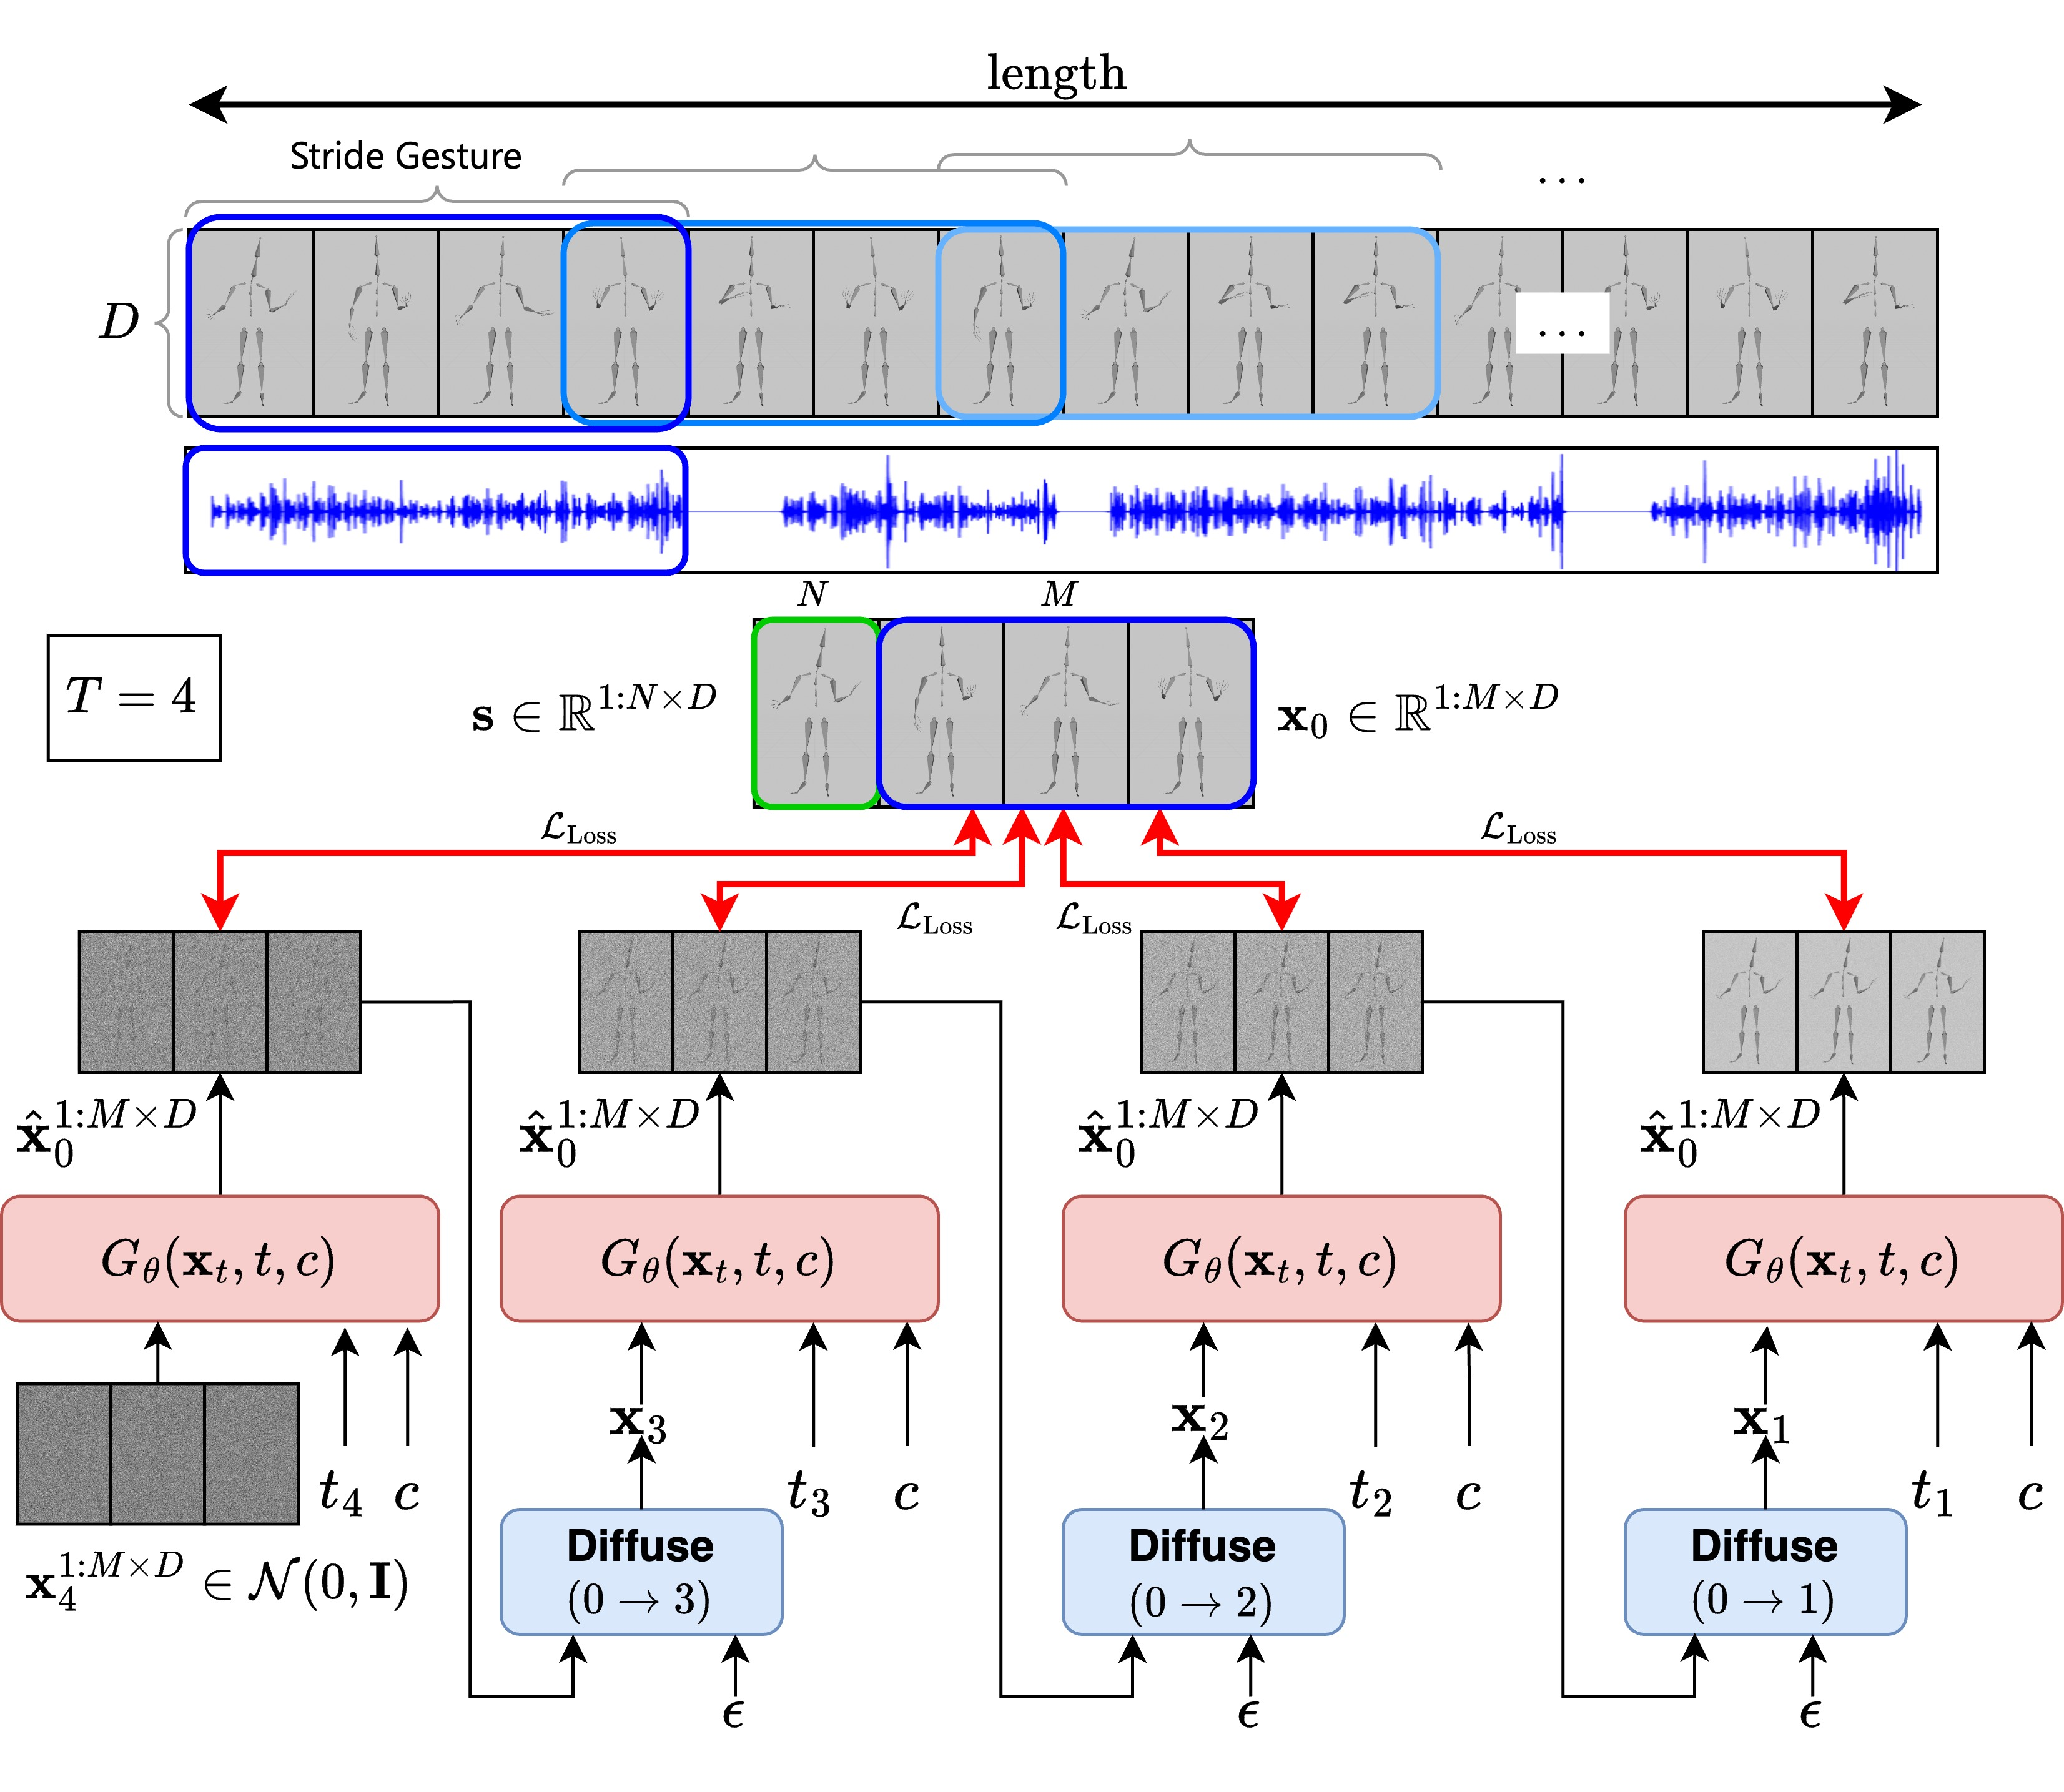
\includegraphics[width=0.8\linewidth]{images/OverviewArchitecture.jpg}
%	\vspace{-10pt}
%	\caption{Kiến trúc OHGesture với $T = 4$}
%	\label{fig:architecturediffusion}
%	\vspace{-10pt}
%\end{figure}


% Ý tưởng của chúng tôi là tạo ra các cử chỉ bằng một mô hình diffusion \cite{ho2020denoising} bằng cách học cách dần dần Denoise từ nhiễu hoàn toàn. Như được thể hiện trong Hình 2, mô hình diffusion bao gồm hai phần: quá trình tiến lùi (quá trình diffusion)  và quá trình ngược lại (quá trình Denoise).

%\subsection{Quá Trình Gây Nhiễu (Diffusion)}
%
%Quá trình diffusion $q$ được mô hình hóa như là một quá trình Markov với đầu vào lần lượt được thêm nhiễu, và sau đó mô hình lần lượt từng bước học để có thể tái tạo lại cử chỉ ban đầu.
%Trong bài toán sinh cử chỉ, đầu vào là các điểm trên tọa độ 3D, gọi là keypoint $x$, với $x_{0} \sim q\left(x_{0}\right)$ và $q\left(x_{0}\right)$ là phân phối của dữ liệu thực tế.
%Trong đó mỗi bước phương sai được thay đổi theo hệ số $\beta_{1}, \beta_{2}, \ldots, \beta_{T}$ $\left(0<\beta_{1}<\beta_{2}<\cdots<\beta_{T}<1, T\right)$, chúng tôi thêm nhiễu Gaussian
%
%\begin{equation} \label{eq:gaussian}
%q\left(x_{t} \mid x_{t-1}\right)=\mathcal{N}\left(x_{t} ; \sqrt{1-\beta_{t}} x_{t-1}, \beta_{t} \mathbf{I}\right)
%\end{equation}
%
%vào cử chỉ tại mỗi thời điểm $t$ lần lượt, và sau khi nhiễu Guassian được thêm vào đến bước $T$ đủ lớn, đến khi kết quả trở nên nhiễu hoàn toàn và không thể phân biệt được với kết quả ban đầu.

%\subsection{Quá Trình Khử Nhiễu (Denoise)}
%
%Quá trình Denoise $p_{\theta}$ là quá trình học tham số $\theta$ thông qua một mạng neural. Giả sử quá trình Denoise cũng tuân theo phân phối Gaussian, tức là nhiễu $x_{t}$ tại thời điểm $t$ được sử dụng để học $\mu_{\theta}, \Sigma_{\theta}$, sau đó
%
%\begin{equation} \label{eq:diffusion}
%p_{\theta}\left(x_{t-1} \mid x_{t}\right)=\mathcal{N}\left(x_{t-1} ; \mu_{\theta}\left(x_{t}, t\right), \Sigma_{\theta}\left(x_{t}, t\right)\right)
%\end{equation}
%
%Để thuận tiện cho việc tính toán, ta cho $\alpha_{t}=1-\beta_{t}$ và viết gọn lại $\bar{\alpha}_{t}=\prod_{i=1}^{T} \alpha_{i}$. Sau đó, cử chỉ nhiễu $x_{t}$ tại thời điểm $t$ có thể được viết lại như sau:
%
%\begin{equation} \label{eq:denoisevariance}
%q\left(x_{t} \mid x_{0}\right)=\mathcal{N}\left(x_{t} ; \sqrt{\bar{\alpha}_{t}} x_{0},\left(1-\bar{\alpha}_{t}\right) \mathbf{I}\right)
%\end{equation}
%
%Mô hình học bằng cách tối ưu hóa bằng cách giảm thiểu sự khác biệt giữa nhiễu thực sự $\epsilon$ và nhiễu được dự đoán $\epsilon_{\theta}\left(x_{t}, t\right)$ \cite{ho2020denoising}. Khi lấy mẫu, chúng ta có thể học giá trị trung bình $\mu_{\theta}\left(x_{t}, t\right)=\frac{1}{\sqrt{\alpha_{t}}}\left(x_{t}-\frac{\beta_{t}}{\sqrt{1-\bar{\alpha}_{t}}} \epsilon_{\theta}\left(x_{t}, t\right)\right)$ với phương sai cố định.

%\subsection{Sinh cử chỉ với điều kiện}
%
%Để tổng hợp $M$ frame cử chỉ  $\bx^{1: M}$  với điều kiện $c$ bao gồm cả cử chỉ khởi tạo, văn bản và âm thanh.
%Tương tự như phương pháp \cite{ramesh2022hierarchical} \cite{tevet2022human}, chúng tôi dự đoán dữ liệu thật $\mathbf{x}_0$ thay vì dự đoán nhiễu $\epsilon_{\theta}\left(x_{t}, t\right)$ như  mô hình diffusion cơ bản \cite{ho2020denoising}. Quá trình khử nhiễu (Denoise) tái tạo dữ liệu gốc $\mathbf{x}_{0}$ dựa trên nhiễu đầu vào $\mathbf{x}_{t}$, bước làm nhiễu $t$ và điều kiện $c$.
%
%\begin{equation} \label{eq:condition}
%\hat{\bx}_{0} = G \left( \bx_{t}, t, c\right)
%\end{equation}
%
%%Để 
%%Chúng tôi sử dụng phương pháp concat đặc trưng âm thanh và văn bản để . Ngoài ra chúng tôi cũng sử dụng phương pháp 
%
%Sau đó, hàm khử nhiễu có thể được huấn luyện bằng cách tối ưu hóa hàm Huber loss \cite{huber1992robust} giữa các cử chỉ dự đoán $\hat{x}_{0}$ và các cử chỉ thực tế $\bx_{0}$ trên các tập huấn luyện:
%
%\begin{equation} \label{eq:huberloss}
%\mathcal{L}=E_{x_{0} \sim q\left(x_{0} \mid c\right), t \sim[1, T]}\left[\operatorname{HuberLoss}\left(\bx_{0}-\hat{\bx}_{0}\right)\right]
%\end{equation}




\subsection{Áp dụng cơ chế Attention cho bài toán sinh cử chỉ}

%\subsection{Hàm xử lý đặc trưng của quá trình khử nhiễu}
%
%Như kiến trúc \textbf{OHGesture} trình bày trong hình \autoref{fig:architecturediffusion}, cử chỉ được tạo ra dựa trên bước làm nhiễu $t$, cử chỉ nhiễu $x_{t}$ và điều kiện $c$ (bao gồm âm thanh $a$, cảm xúc $s$ và cử chỉ khởi tạo $d$ ). Đối với mỗi đặc trưng, quá trình sinh cử chỉ được xử lý như sau:


%\subsection{Cơ chế Attention trong hàm khử nhiễu}

Mục tiêu của việc áp dụng cơ chế attention trong mô hình của chúng tôi là mô hình có thể hiểu được mối liên hệ của từng khung hình với nhau, vì vậy phương pháp của chúng tôi là biểu diễn các đặc trưng của từng khung hình bằng các vector đặc trưng riêng lẻ, và với từng đặc trưng của khung hình riêng lẻ, chúng tôi mong muốn tìm được sự tương quan và mối quan hệ giữa các đặc trưng với nhau.
Như hình minh hoạ \ref{fig:OHGesture}, sau quá trình trích xuất đặc trưng. Để tính được sự tương quan của các đặc trưng xa, chúng tôi sẽ học để biểu diễn được các ngữ cảnh cực bộ (local context) theo \cite{rae2020transformers}.


% mà chúng tôi chọn trong mô hình diffusion
Đầu tiên cử chỉ khởi tạo $\mathbf{S}$ và vector cảm xúc $\mathbf{E}$ được ghép lại với nhau để tạo thành một vectơ có kích thước $256$, bởi vì kích thước $256$ là kích thước vector tiềm ẩn. Sau đó được cộng thêm vector timestep $\mathbf{T}$ để tạo thành vector $\mathbf{Z}$. Vector $\mathbf{Z}$ thể hiện thông tin chúng tôi thực sự muốn điều khiển bằng diffusion có điều kiện.

Để có thể căn chỉnh văn bản, âm thanh tương đồng với từng khung hình cử chỉ, chúng tôi sẽ concat các đặc trưng âm thanh, văn bản và cử chỉ đồng thời với nhau. Sau đó để căn chỉnh theo miền thời gian các đặc trưng về cảm xúc và cử chỉ khởi tạo chúng tôi sẽ copy vector $\mathbf{Z}$ để các bản sao của nó được ghép thành một chuỗi vector đặc trưng tương đồng với $M$ khung hình. Sau đó đưa vào lớp local attention (chú ý cục bộ). Tương tự ý tưởng từ phương pháp Routing Transformer \cite{roy2021efficient}, local attention cho thấy rằng sự quan trọng trong việc xây dựng biểu diễn các vector đặc trưng trung gian. Các vector đặc trưng sẽ được cộng thêm một vector sinusoids hay mã hoá vị trí tương đối (Relative position encoding \cite{vaswani2017attention}) để thể hiện được đặc trưng thời gian trước khi đi qua lớp Cross-Local Attention
%mà cho thấy rằng 

%Sau đó, vectơ $\mathbf{Z}$ và các bản sao của nó được ghép thành một chuỗi vector đặc trưng để khớp với dòng thời gian của âm thanh và đặc trưng cử chỉ, sau đó ghép với âm thanh $\mathbf{A}$ và cử chỉ $\mathbf{G}$ để làm đầu vào cho 
%Phương pháp sinh cử chỉ song hành với âm thanh của chúng tôi sử dụng lớp Local Attention được lấy ý tưởng từ 

\begin{equation} \label{eq:attention}
	\operatorname{Attention}(\mathbf{Q}, \mathbf{K}, \mathbf{V}, \mathbf{M})=\operatorname{softmax}\left(\frac{\mathbf{Q} \mathbf{K}^{T}+\mathbf{M}}{\sqrt{C}}\right) \mathbf{V}
\end{equation}

Công thức Attention trên có $\mathbf{Q}$, $\mathbf{K}$ ,$\mathbf{V}$ là các ma trận sau khi đi qua các ma trận biến đối tuyến tính $\mathbf{Q} = \mathbf{X} \mathbf{W}_Q$, $\mathbf{K} = \mathbf{X} \mathbf{W}_K$, $\mathbf{V} = \mathbf{X} \mathbf{W}_V$. Với đầu vào là ma trận biểu thị chuỗi $M$ khung hình, với mỗi khung hình là một vector được concat từ các vector đặc trưng bao gồm cả cử chỉ khởi tạo, văn bản, âm thanh, cảm xúc và cử chỉ $\bx_t$ mà chúng tôi muốn thực hiện khử nhiễu. Quá trình Local-Cross Attention được điều khiển chỉ để tính các đặc trưng cục bộ của chuyển động của các cử chỉ và đặc trưng trong các khung hình lân cận.

Hàm Attention hoạt động như một bộ từ điển, với các thông tin cuối cùng tra được là ma trận $\mathbf{V}$ (value), còn $\mathbf{Q}$ (query) là từ khoá muốn tìm kiếm, $\mathbf{K}$ (key) là danh mục các từ khoá trong bộ từ điển tra cứu. Quá trình Attention sẽ tính toán mức độ tương đồng giữa \( \mathbf{Q} \) và \( \mathbf{K} \) để xác định trọng số cho các giá trị trong \( \mathbf{V} \). Kết quả cuối cùng là tổ hợp các giá trị trong \( \mathbf{V} \), trong đó các giá trị tương ứng với các khoá giống truy vấn nhất sẽ có trọng số cao hơn. $\mathbf{M}$ là mặt nạ (mask) để thực hiện quá trình chú ý cục bộ.

%\begin{equation}
%\begin{aligned}
%	\text{MultiHeadAttn}(\mathbf{X}_q, \mathbf{X}_k, \mathbf{X}_v) &= [\text{head}_1; \dots; \text{head}_h] \mathbf{W}^o \\ 
%	\text{where head}_i &= \text{Attention}(\mathbf{X}_q\mathbf{W}^q_i, \mathbf{X}_k\mathbf{W}^k_i, \mathbf{X}_v\mathbf{W}^v_i)
%\end{aligned}
%\end{equation}


Sau quá trình Cross-Local Attention, mô hình tiếp tục được đưa qua lớp tuyến tính để căn chỉnh tương ứng với $M$ khung hình, bao gồm $\mathbf{h}^{1:M}$.
Sau đó quá trình tương tự như xử lý các vector đặc trưng của mô hình BERT \cite{devlin2019bertpretrainingdeepbidirectional} văn bản. Chúng tôi sử dụng $z$ là $\mathbf{Z} \in \mathbb{R}^{256}$ token đầu tiên biểu thị đặc trưng biểu thị cho toàn bộ chuỗi $M$ khung hình. 
Các vector $\mathbf{h}$ biểu thị cho chuỗi $M$ khung hình, tương tự như phương pháp Reformer \cite{kitaev2020reformer}, trước khi đi vào lớp self-attention trong Transformer Encoder, mô hình sẽ sử dụng lớp mã hoá vị trí tương đối (Relative Position Encoding - RPE) để thay thế mã hoá vị trí tuyệt đối, giúp mô hình hiệu quả hơn trong việc xử lý chuỗi dài.
Khi vào lớp Transformer Encoder \cite{vaswani2017attention} giúp tính toán được mối liên hệ giữa các chuỗi dữ liệu. Trong lớp Transformer Encoder mô hình sẽ áp dụng cơ chế tự chú ý tương tự như trên nhưng không sử dụng mặt nạ. 
%Để yếu tố thời gian không ảnh hưởng nhiều đến kết quả sinh cử chỉ, chúng tôi sử dụng cơ chế mã hóa vị trí tương đối 
Cuối cùng, đầu ra của self-attention được ánh xạ lại cùng kích thước như $\bx_{0}$ sau một lớp biến đổi tuyến tính. Mục tiêu của toàn bộ mô hình $G_\theta ( \mathbf{x}_t, t, c )$ là để học được trọng số $\theta$, với quá trình denoise sẽ giảm dần từ $t = T$ đến khi $t = 1$ ta thu được $\bx_0$.
%Các cơ chế attention khác nhau có thể được tạo ra bằng cách điều chỉnh lớp mask tương ứng $\mathbf{M}$.

%\begin{figure*}[ht]
%\begin{minipage}[b]{0.25\textwidth}
%\centering
%    [width=\textwidth]{images/attention_full.jpg}
%    \caption*{(a) full self-attention}
%\end{minipage}
%\hfill
%\begin{minipage}[b]{0.25\textwidth}
%\centering
%    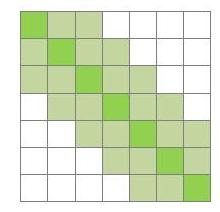
\includegraphics[width=\textwidth]{images/attention_sidewindow.jpg}
%    \caption*{(b) sliding window attention}
%\end{minipage}
%\hfill
%\begin{minipage}[b]{0.25\textwidth}
%\centering
%    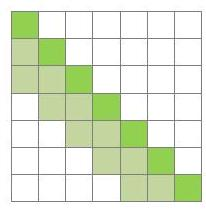
\includegraphics[width=\textwidth]{images/cross_attention.jpg}
%    \caption*{(c) cross-local attention}
%\end{minipage}
%% \label{fig:type_attention}
%\caption[Các loại attention khác nhau (full self-attention, sliding window attention, cross-local attention)]{Các loại attention khác nhau được sử dụng trong các thí nghiệm của chúng tôi, trong đó (a) và (c) là cơ chế attention được sử dụng trong mô hình của chúng tôi và (b) là một mẫu được sử dụng để đánh giá trong thực nghiệm. Mỗi dòng tương ứng với input và mỗi cột tương ứng với output của mô hình}
%\end{figure*}

\begin{figure}[H]
	\centering
	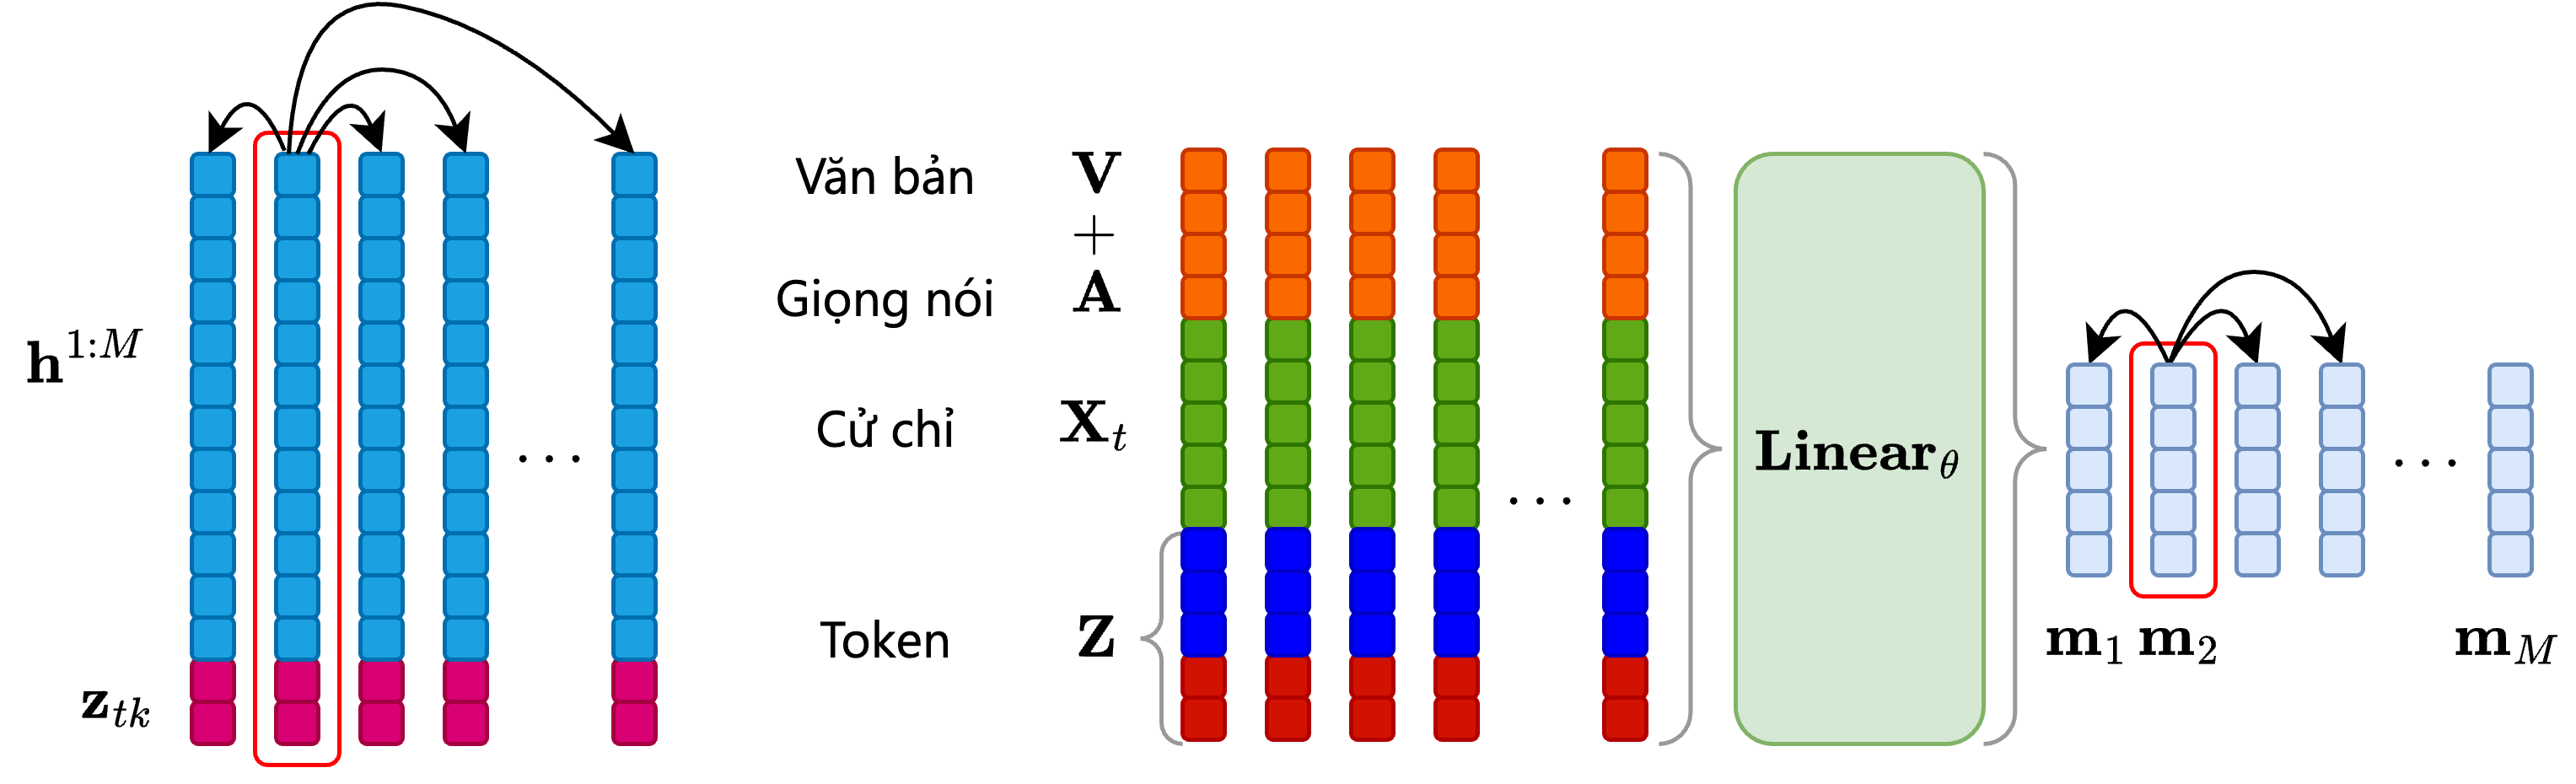
\includegraphics[width=0.6\textwidth]{CrossLocalAttention}
	\caption{Cơ chế Self-Attention trong Transformer Encoder và Cross-Local Attention}
	\label{fig:CrossLocalAttention}
\end{figure}


% Phần 4.3. Các hàng đại diện cho các đầu ra và các cột đại diện cho đầu vào. Các hình vuông màu sáng tô màu cho các phần tử liên quan đến mỗi dòng đầu ra.



%tương tự như phương pháp Longformer \cite{beltagy2020longformer} chúng tôi cũng thử nghiệm cơ chế \textit{sliding window attention}.

%\subsection{Phương pháp sample cử chỉ}


%như kiến trúc trong phần 
%\autoref{fig:architecturediffusion}.


% chúng tôi , trong mỗi bước làm nhiễu $t$, chúng tôi dự đoán cử chỉ sạch  $=$  $\left(x_{t}, t, c\right)$, và thêm nhiễu vào bước làm nhiễu $x_{t-1}$ sử dụng Phương trình (1) với quá trình trải đều. Quá trình này được lặp lại từ $t=T$ cho đến khi đạt được $x_{0}$ (Hình 2 dưới cùng).

\subsection{Điều khiển cảm xúc trong bài toán sinh cử chỉ}

Ở các bước trên mô hình đã có thể học được cách sinh cử chỉ, nhưng để mô hình có thể học được các cảm xúc ở các tình huống khác nhau sẽ được giải quyết bằng cách tham số hóa và lần lượt thay đổi từng cảm xúc để sao cho khi thay đổi cảm xúc thì kết quả dự đoán phải có cảm xúc tương ứng.

Tương tự như các phương pháp sử dụng mô hình khử nhiễu có điều kiện \cite{ho2022classifier}, \cite{tevet2022human}, chúng tôi sử dụng điều kiện $c = [ \mathbf{s}, \mathbf{e}, \mathbf{a}, \mathbf{v} ]$,  bao gồm cử chỉ khởi tạo $\mathbf{s}$, cảm xúc $\mathbf{e}$, âm thanh tương ứng $\mathbf{a}$ và văn bản $\mathbf{v}$. Mô hình diffusion có điều kiện $c$ ở đây sẽ là tổng cả trường hợp ở từng bước $t$ trong mô hình khử nhiễu $\text{G}_\theta \left( \bx_{t}, t, c \right)$, với  $c_{\varnothing}=[\varnothing, \varnothing, \mathbf{a}, \mathbf{v}]$ không điều kiện và $c = [\mathbf{s}, \mathbf{e}, \mathbf{a}, \mathbf{v}]$ có điều kiện. Quá trình này có thể dễ dàng điều khiển bằng một lớp mặt nạ ngẫu nhiên (random mask) trên các vector đặc trưng của cử chỉ khởi tạo $\mathbf{s}$ và cảm xúc $\mathbf{e}$. Khi đó, mô hình chỉ việc thay đổi nhãn tương ứng với lớp mask đã lấy ngẫu nhiên để mô hình có thể tối ưu theo các điều kiện khác nhau. 

%Khi đó hàm khử nhiễu $\text{G}_\theta \left( \bx_{t}, t, c_{1}\right), c_{1}=[\mathbf{s}, \mathbf{e}, \mathbf{a}, \mathbf{v}]$ và hàm khử nhiễu mà không có điều kiện $\text{G}_\theta \left( \bx_{t}, t, c_{2}\right), c_{2}=[\varnothing, \varnothing, \mathbf{a}, \mathbf{v}]$ sẽ được tối ưu trong quá trình huấn luyện, theo công thức

\begin{equation} \label{eq:denoise}
\hat{x}_{0 c, c_{\varnothing}, \gamma}=\gamma G \left(x_{t}, t, c\right)+(1-\gamma) G \left(x_{t}, t, c_{\varnothing}\right)
\end{equation}

Điểm đặc biệt là ta có thể dựa trên việc học có điều kiện và không có điều kiện của classifier-free guidance \cite{ho2022classifier}, ta có thể nội suy giữa hai cảm xúc $\mathbf{e}_1$ và cảm xúc $\mathbf{e}_2$ khác nhau bằng cách cho điều kiện $c = \left[\mathbf{s}, \mathbf{e}_{1}, \mathbf{a}, \mathbf{v} \right]$ và $c_\varnothing = \left[\mathbf{s}, \mathbf{e}_{2}, \mathbf{a}, \mathbf{v} \right]$. Khi đó ta có thể viết lại $\hat{x}_{0 \gamma, c_{1}, c_{2}}=\gamma G \left(x_{t}, t, c_{1} \right)+(1-\gamma) G \left(x_{t}, t, c_{2}\right)$.
%Trong thực tế, hàm Denoise học cả phân phối có điều kiện và không có điều kiện bằng cách ngẫu nhiên phần mask $10 \%$ của các mẫu bằng các mask theo phân phối Bernoulli. Sau đó, đối với kiểu $s$ trong điều kiện, chúng ta có thể tạo ra cử chỉ được kiểm soát kiểu khi lấy mẫu bằng cách nội suy hoặc thậm chí là dự đoán hai biến thể bằng cách sử dụng $\gamma$, như $c_{1}=\left[s, e_{1}, a, v \right], c_{2}=\left[s, e_{2}, a, v \right]$


\subsection{Quá trình huấn luyện}

Thuật toán huấn luyện mô hình OHGesture bắt đầu bằng việc tính toán các giá trị và siêu tham số cần thiết như $\gamma$, $\sqrt{\alpha_t}$, $\sqrt{1 - \alpha_t}$, $\sqrt{\bar{\alpha}_t}$ và nhiễu ngẫu nhiên $\boldsymbol{\epsilon}_t$ cho từng bước thời gian $t$ từ 1 đến $T$. Sau đó, nhãn ban đầu $\mathbf{x}_0$, đại diện cho cử chỉ gốc, được lấy từ phân phối dữ liệu đã chuẩn hóa. Tiếp theo, các mặt nạ Bernoulli $c_1$ và $c_2$ được tạo ngẫu nhiên, mô phỏng các điều kiện khác nhau như cử chỉ, cảm xúc, âm thanh, hoặc văn bản, với một trong các mặt nạ có thể là không có thông tin cảm xúc. Sau khi có các mặt nạ, nhiễu được thêm vào để tạo thành cử chỉ nhiễu $\mathbf{x}_t$, được tính bằng công thức kết hợp chuỗi cử chỉ gốc và nhiễu ngẫu nhiên. Quá trình tiếp theo là chọn ngẫu nhiên một bước thời gian $t$ trong khoảng $[1, T]$ và sử dụng cử chỉ nhiễu $\mathbf{x}_t$ cùng các mặt nạ để dự đoán lại chuỗi cử chỉ gốc thông qua mô hình, trong đó dự đoán được tính bằng một sự kết hợp của các hàm tạo ra từ các điều kiện mặt nạ. Sau khi có dự đoán, loss được tính bằng cách sử dụng HuberLoss giữa chuỗi cử chỉ gốc và dự đoán, từ đó đạo hàm loss để cập nhật các tham số trọng số $\theta$. Quá trình huấn luyện này được lặp lại cho đến khi mô hình hội tụ và thu được các tham số tối ưu $\theta'$.


\begin{algorithm}[H]
	\caption{Thuật toán huấn luyện}
	\setlength{\baselineskip}{10pt}
	\begin{enumerate}
		\item Tính sẵn các giá trị và siêu tham số: $\gamma$, $\sqrt{\alpha_t}$, $\sqrt{1 - \alpha_t}$, $\sqrt{\bar{\alpha}_t}$ và nhiễu ngẫu nhiên $\boldsymbol{\epsilon}_t$ tại mỗi bước $t: 1 \rightarrow T$. Định nghĩa lịch nhiễu $\{\alpha_t \in (0, 1)\}_{t=1}^T$.
		
		\item Lấy nhãn ban đầu $\mathbf{x}_0$ từ phân phối dữ liệu đã chuẩn hóa.
		
		\item Random các mặt nạ Bernoulli $c_{1} = \big[ \mathbf{s}, \mathbf{e_1}, \mathbf{a}, \mathbf{v} \big]$, $c_{2} = \big[ \mathbf{s}, \mathbf{e_2}, \mathbf{a}, \mathbf{v} \big]$, hoặc $c_{2} = \big[ \varnothing, \varnothing, \mathbf{a}, \mathbf{v} \big]$.
		
		\item Thêm nhiễu để có cử chỉ nhiễu $\mathbf{x}_t$:
		\[
		\mathbf{x}_t = \sqrt{\bar{\alpha}_t} \mathbf{x}_0 + \sqrt{1 - \bar{\alpha}_t} \boldsymbol{\epsilon}_t
		\]
		
		\item Với mỗi bước $t$, lấy \textbf{ngẫu nhiên} $t$ từ $[1, T]$.
		
		\item Với $\mathbf{x}_t$, $t$ và các điều kiện mặt nạ $c_1$, $c_2$, dự đoán chuỗi cử chỉ:
		\[
		\hat{\mathbf{x}}_{0 \gamma, c_{1}, c_{2}} = \gamma G_{\theta} \left(\mathbf{x}_{t}, t, c_{1}\right) + (1 - \gamma) G_{\theta} \left(\mathbf{x}_{t}, t, c_{2}\right)
		\]
		
		\item Tính loss và đạo hàm để cập nhật trọng số $\theta$:
		\[
		\mathcal{L}_t = \mathbb{E}_{t \sim [1, T], \mathbf{x}_0, \boldsymbol{\epsilon}_t} \left[ \operatorname{HuberLoss}(\mathbf{x}_0, \hat{\mathbf{x}}_0 ) \right]
		\]
		
		\item Lặp lại từ bước 6 cho đến khi hội tụ, thu được các tham số tối ưu $\theta'$.
	\end{enumerate}
\end{algorithm}

%
%
%\begin{enumerate}
%	\item Tính sẵn các giá trị, và các siêu tham số: $\gamma$, $\sqrt{\alpha_t}$ $\sqrt{1 - \alpha_t}$, $\sqrt{\bar{\alpha}_t}$, Random nhiễu $\bepsilon_t$ ở mọi bước $t: 1 \rightarrow T$.
%	$\{\alpha_t \in (0, 1)\}_{t=1}^T$
%	\item Lấy nhãn $\bx_0$ từ phân bố của dữ liệu đã chuẩn hoá
%	\item Random Bernoulli masks  $c_{1} = \big[ \mathbf{s} , \mathbf{e_1}, \mathbf{a}, \mathbf{v} \big]$, $c_{2} = \big[ \mathbf{s} , \mathbf{e_2}, \mathbf{a}, \mathbf{v}\big]$ hoặc $c_{2} = \big[ \varnothing , \varnothing, \mathbf{a},  \mathbf{v} \big]$
%	\item Forward $\bx_0$ để có cử chỉ nhiễu $\mathbf{x}_t$ :  $\mathbf{x}_t = \sqrt{\bar{\alpha}_t}\mathbf{x}_0 + \sqrt{1 - \bar{\alpha}_t}\boldsymbol{\epsilon}_t$
%	\item $\text{for all}$ $t$, lẫy $t$ \textbf{ngẫu nhiên} $t \sim [1, T]$
%	\item Cho $\bx_t$ và $t$, $c$, $c_{\varnothing}$ để dự đoán chuỗi cử chỉ
%	\begin{equation}
%		\hat{\mathbf{x}}_{0 \gamma, c_{1}, c_{2}}=\gamma G_{\theta} \left(\mathbf{x}_{t}, t, c_{1}\right)+(1-\gamma) G_{\theta} \left(\mathbf{x}_{t}, t, c_{2}\right)
%	\end{equation}
%	\item Tính loss và đạo hàm để cập nhật trọng số $\theta$
%	\begin{equation}
%		\mathcal{L}_t = \mathbb{E}_{t \sim [1, T], \mathbf{x}_0, \boldsymbol{\epsilon}_t} \Big[ \operatorname{HuberLoss}(\mathbf{x}_0, \hat{\mathbf{x}}_0 ) \Big]
%	\end{equation}
%	
%	\item Quay lại bước 6 cho đến khi hội tụ để thu được $\theta'$
%\end{enumerate}


\subsection{Quá trình lấy mẫu}

Để có thể sinh cử chỉ với chiều dài tùy ý, chúng tôi cắt chuỗi ban đầu thành các đoạn ngắn có chiều dài $M$. Trong quá trình huấn luyện, cử chỉ khởi tạo đầu tiên có thể được tạo ra bằng cách lấy ngẫu nhiên cử chỉ từ tập dữ liệu hoặc từ lấy trung bình từ đoạn cắt được. Cụ thể ở đây, sẽ lấy góc quay trung bình trong các đoạn đã cắt được. Tiếp theo chúng ta chỉ việc lấy lần lượt các frame đã sinh ra và chọn $N = 8$ frame cuối cùng làm cử chỉ khởi tạo ở lượt tiếp theo. Đối với mỗi đoạn đã cắt ra, cử chỉ $\bx_{t}$ lần lượt sẽ được áp dụng hàm khử nhiều $\hat{\bx}_{0} = G_{\theta'} \left( \bx_{t}, t, c\right)$, sau khi có $\hat{\bx}_{0}$ ta sẽ Diffuse (thêm nhiễu) cho đến khi được  $\bx_{t-1}$, và $\bx_{t-1}$ sẽ tiếp tục được làm khử nhiễu cho đến bước khử nhiễu $t=1$ sẽ đạt được $\bx_{0}$ 

\begin{algorithm}
	\caption{Thuật toán lấy mẫu (sampling)}
	\setlength{\baselineskip}{10pt}
	\begin{enumerate}
		\item Khởi tạo với nhiễu: $\mathbf{x}_T \sim \mathcal{N}(0, \mathbf{I})$.
		
		\item Các giá trị $\sqrt{\alpha_t}$, $\sqrt{1 - \alpha_t}$ và $\sqrt{\bar{\alpha}_t}$ lấy từ quá trình huấn luyện, tính sẵn giá trị $\sigma_t$ từ $\alpha_t$ ở mỗi bước $t: 1 \rightarrow T$.
		
		\item Chia mỗi đoạn âm thanh 4 giây thành: $\mathbf{a} \in \mathbb{R}^{64000}$. Cử chỉ khởi tạo $\mathbf{s}$ ban đầu là trung bình dữ liệu, sau đó được lấy từ đoạn cử chỉ đã suy luận. Chọn cảm xúc mong muốn, văn bản được lấy từ âm thanh chuyển mã $\mathbf{a}$, tạo cặp điều kiện $c = [\mathbf{s}, \mathbf{e}, \mathbf{a}, \mathbf{v}]$.
		
		\item Với mỗi $t$, lấy $t$ \textbf{tuần tự} từ $[T, \dots, 1]$.
		
		\item Tạo nhiễu ngẫu nhiên $\mathbf{z} \sim \mathcal{N}(0, \mathbf{I})$.
		
		\item Đưa $\mathbf{x}_t$ vào để suy luận $\hat{\mathbf{x}}_0^{(t)} = G_{\theta'}(\mathbf{x}_t, t, c)$.
		
		\item Chuyển tiếp $\hat{\mathbf{x}}_0^{(t)}$ từ bước $0 \rightarrow t$ để nhận $\hat{\mathbf{x}}_{t-1}^{(t)}$.
		
		\item Cộng thêm nhiễu: $\hat{\mathbf{x}}_{t-1} = \hat{\mathbf{x}}_{t-1}^{(t)} + \sigma_t \mathbf{z}$.
		
		\item Quay lại bước 4. Khi $t = 1$, thu được $\hat{\mathbf{x}}_0$ từ quá trình khử nhiễu.
	\end{enumerate}
	\label{alg:sampling}
\end{algorithm}

Thuật toán \ref{alg:sampling} lấy mẫu bắt đầu bằng việc khởi tạo cử chỉ nhiễu ban đầu $\mathbf{x}_T$ từ phân phối chuẩn $\mathcal{N}(0, \mathbf{I})$. Sau đó, các giá trị $\sqrt{\alpha_t}$, $\sqrt{1 - \alpha_t}$ và $\sqrt{\bar{\alpha}_t}$ được lấy từ quá trình huấn luyện, cùng với giá trị $\sigma_t$ được tính từ $\alpha_t$ tại mỗi bước thời gian $t$ từ 1 đến $T$. Mỗi đoạn âm thanh 4 giây được chia thành các chuỗi dữ liệu $\mathbf{a}$, và cử chỉ khởi tạo $\mathbf{s}$ được lấy từ trung bình dữ liệu hoặc từ đoạn cử chỉ đã suy luận. Cảm xúc mong muốn và văn bản được lấy từ âm thanh chuyển mã $\mathbf{a}$, tạo thành một cặp điều kiện $c = [\mathbf{s}, \mathbf{e}, \mathbf{a}, \mathbf{v}]$. Thuật toán sau đó thực hiện các bước tuần tự, bắt đầu từ bước cuối cùng $T$ và tiến ngược về 1. Ở mỗi bước, nhiễu ngẫu nhiên $\mathbf{z}$ được tạo ra và mô hình dự đoán $\hat{\mathbf{x}}_0^{(t)}$ từ cử chỉ nhiễu $\mathbf{x}_t$, thời gian $t$, và cặp điều kiện $c$. Dự đoán này được chuyển tiếp để tính toán $\hat{\mathbf{x}}_{t-1}^{(t)}$ cho bước tiếp theo, và nhiễu được cộng vào để cập nhật cử chỉ tại bước $t-1$. Quá trình này lặp lại cho đến khi đạt đến bước 1, khi đó thuật toán thu được cử chỉ khử nhiễu $\hat{\mathbf{x}}_0$ là kết quả dự đoán cuối cùng.


%\begin{enumerate}
%	\item Bắt đầu với nhiễu: $\bx_T \sim \mathcal{N}(0, \mathbf{I})$
%	\item Các giá trị $\sqrt{\alpha_t}$ $\sqrt{1 - \alpha_t}$ và $\sqrt{\bar{\alpha}_t}$ có được từ bước huấn luyện, tính sẵn các giá trị  $\sigma_t$ từ $\alpha_t$ ở mọi bước $t: 1 \rightarrow T$
%	\item Cắt mỗi 4s âm thanh thành: $\mathbf{a} \in \mathbb{R}^{64000}$, cử chỉ khởi tạo $\mathbf{s}$ ban đầu là trung bình dữ liệu, sau đó được lấy từ đoạn cử chỉ đã suy luận. Chọn cảm xúc mong muốn, văn bản được lấy từ transribe speech $\mathbf{a}$ và tạo cặp condition $c = [\mathbf{s}, \mathbf{e}, \mathbf{a},  \mathbf{v}]$
%	\item $\text{for all}$ $t$, lấy $t$ \textbf{tuần tự} $t \sim [T, \dots 1]$
%	\item Random nhiễu $\bz \sim \mathcal{N}(0, \mathbf{I})$
%	\item Đưa $\bx_t$ vào để suy luận $\hat{\bx}_0^{(t)} = G_{\theta'}(\bx_t, t, c)$
%	\item Forward $\hat{\bx}_0^{(t)}$ $0 \rightarrow t$ để được $\hat{\bx}_{t-1}^{(t)}$
%	\item Cộng thêm một lượng nhiễu $\hat{\bx}_{t-1} = \hat{\bx}_{t-1}^{(t)} + \sigma_t \bz$
%	\item Quay lại bước $4$, khi $t=1$ ta thu được $\hat{\bx}_0$ từ quá trình khử nhiễu
%\end{enumerate}

% \begin{figure*}[ht]
% \begin{minipage}[b]{0.3\textwidth}
% \centering
%     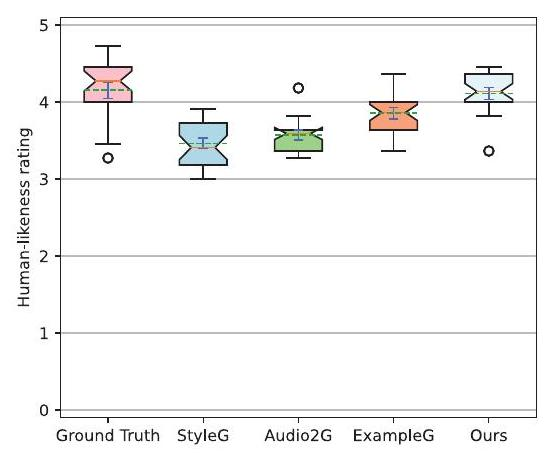
\includegraphics[width=\textwidth]{images/humanlike_score.jpg}
%     \caption*{(a) Biểu đồ hộp của đánh giá về tính giống với con người}
% \end{minipage}
% \hfill
% \begin{minipage}[b]{0.3\textwidth}
% \centering
%     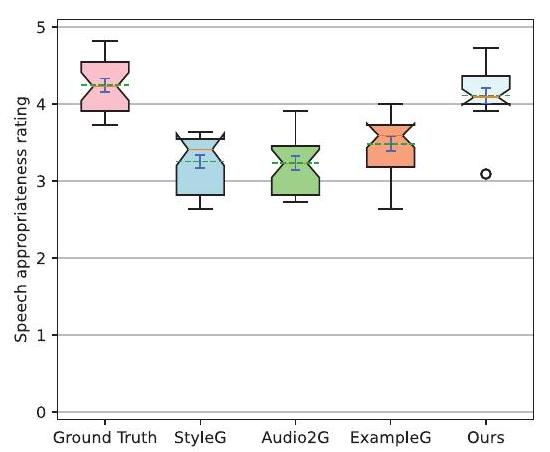
\includegraphics[width=\textwidth]{images/speech_score.jpg}
%     \caption*{(b) Biểu đồ hộp của đánh giá về tính phù hợp giữa cử chỉ và âm thanh.}
% \end{minipage}
% \hfill
% \begin{minipage}[b]{0.3\textwidth}
% \centering
%     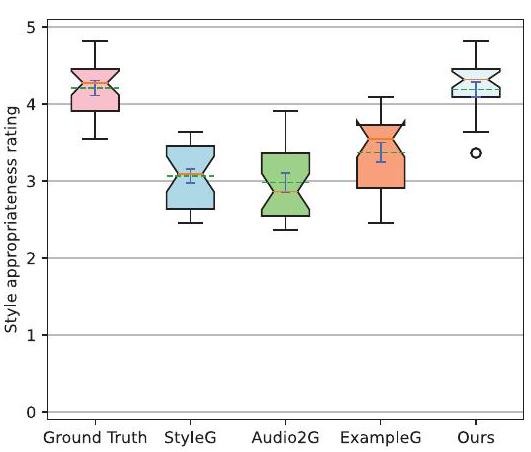
\includegraphics[width=\textwidth]{images/style_score.jpg}
%     \caption*{(c) Biểu đồ hộp của đánh giá về tính phù hợp giữa cử chỉ và cảm xúc}
% \end{minipage}
% \label{fig:gesture_score}
% \caption{Biểu đồ hộp mô tả kết quả so sánh MOS cho các mô hình khác nhau trong các chiều khác nhau. Hộp mở rộng từ phân vị thứ nhất thấp nhất (Q1) đến phân vị thứ ba lớn nhất (Q3) của dữ liệu. Đường đỏ chỉ là giữa. Các khe nhỏ biểu thị khoảng tin cậy $95\%$ (CI) xung quanh giữa. Khi CI nhỏ hơn Q1 hoặc lớn hơn Q3, khe mở rộng ra khỏi hộp, tạo ra một hình dáng "lật" độc đáo. Chúng tôi cũng đã đánh dấu giá trị trung bình và khoảng tin cậy $95\%$ của nó trong hình với đường nét đứt màu xanh lá cây và đường dọc màu xanh lam, tương ứng.}
% \end{figure*}


% Hình 4: Biểu đồ hộp thể hiện kết quả so sánh của MOS cho các mô hình khác nhau trong các chiều không gian khác nhau. Hộp mở rộng từ phần tư dưới thứ nhất (Q1) đến phần tư lớn thứ ba (Q3) của dữ liệu. Đường đỏ chỉ ra trung vị. Các rãnh biểu thị khoảng tin cậy $95 \%$ (CI) xung quanh trung vị. Khi CI ít hơn Q1 hoặc lớn hơn Q3, rãnh mở rộng ra ngoài hộp, tạo cho nó một diện mạo "lật" độc đáo. Chúng tôi cũng đã đánh dấu giá trị trung bình và CI $95\%$ của nó trong hình với một đường kẻ xanh lá cây đứt và một đường kẻ đứt màu xanh dương, tương ứng.

% \begin{equation}
% \left[\mathbf{r}_p, \mathbf{r}_r, \dot{\mathbf{r}}_p, \dot{\mathbf{r}}_r, \rho_p, \rho_r, \dot{\rho}_p, \dot{\rho}_r, g_d\right]
% \end{equation}


% Mô hình OHGesture được dựa trên mô hình QPGesture \cite{yang2023qpgesture} với nền tảng chính của phương pháp dựa trên mô hình VQ-VAE là mã hóa (encode) và giải mã (decode) dữ liệu hay nói cách khác chúng ta sẽ biểu diễn toàn bộ dữ liệu ở chiều dữ liệu thấp hơn và sau đó biểu diễn ngược trở lại kích thước ban đầu. Dữ liệu được biểu diễn thành các vùng trong không gian, với mỗi vùng có một đại diện tương ứng. Từ các địa diện ta có thể mã hóa ngược trở lại để chọn ra các ứng viên cử chỉ theo ngữ nghĩa (dữ liệu văn bản) hoặc nhịp điệu lời nói (dữ liệu âm thanh).
% Dựa trên hai cử chỉ ứng viên (gesture candidate), ta trích xuất ra pha dựa trên vận tốc xoay của các các khớp khi di chuyển và dựa trên pha hiện tại của cử chỉ khởi tạo, ta sẽ chọn được cử chỉ có pha gần nhât hay phù hợp nhất để chọn ra chuỗi cử chỉ cuối cùng.

% Cụ thể quá trình huấn luyện của mô hình bao gồm các quá trình như sau: Lượng tử hóa (Quantization), Ghép các chuyển động cử chỉ (Motion Matching), Điều hướng dựa theo pha của cử chỉ (Phrase Guided).

% Kiến trúc mô hình được trình bày minh họa trong hình \autoref{fig:architecturediffusion}.








% \subsection{Lượng tử hóa (Quantization)}
% % Learning a discrete latent space representation

% Lượng tử hóa là việc học để biểu diễn dữ liệu trong không gian rời rạc (discrete latent space representation). Ta sẽ biểu diễn dữ liệu lên không gian tiềm ần (latent space).
% Mục tiêu của việc lượng tử hóa là biểu diễn dữ liệu dưới số chiều thấp hơn hay chấm điểm/đánh giá dựa trên các đặc trưng của dữ liệu, từ đó dùng các điểm đã đánh giá để so sánh với nhau. Sau khi so sánh đánh giá, ta chọn được một ứng viên tốt nhất, từ ứng viên tốt nhất ta sẽ học để giải mã (decode) ngược trở lại dữ liệu ban đầu.

% Dữ liệu đầu vào được lượng tử hóa bao gồm âm thanh, cử chỉ và văn bản. Trong bài toán sinh cử chỉ, chúng tôi chỉ tập trung vào việc xử lý dữ liệu dựa trên cử chỉ nên đôi với dữ liệu văn bản và âm thanh, ta chỉ sử dụng lại các mô hình pre-train có sẵn. Với âm thanh chúng tôi sử dụng mô hình VQ-Wave2Vec \cite{baevski2019vq} để biểu diễn các dữ liệu âm thanh thành các latent vector. Hàm lượng tử hóa âm thanh là hàm $f_{quant\_audio} : \mathbf{A} \mapsto \mathbf{Z_{audio}}$ trong đó $\textbf{A}$ là các chuỗi các âm thanh sẽ được mã hóa lên vector lantent $\textbf{Z}$. Với $\textbf{Z_{audio}} \in \mathcal{Z}_a$.

% Đối với văn bản, chúng tôi sử dụng mô hình Sentene BERT \cite{reimers2019sentence} để biểu diễn các dữ liệu văn bản thành các vector tiềm ẩn. Hàm để nhúng các dữ liệu văn bản thành các vector là hàm $f_{embedding\_text} : \mathbf{T} \mapsto \mathbf{Z_{text}}$.

% Với cử chỉ, mô hình dựa trên kiến trúc của mô hình VQ-VAE. Hàm lượng tử hóa cử chỉ là hàm $f_{quant\_gesture} : \mathbf{G} \mapsto \mathbf{Z_{gesture}}$ với $\textbf{G}$ là các vector trong codebook $\mathcal{Z_g}$

% % Sau đó dựa trên các điểm dữ liệu trước đó để tìm được đại diện phù hợp trong các vùng.
% % Dựa trên chuỗi các dữ liệu đại diện ta có thể tìm được chuỗi các pha của cử chỉ và từ đó chọn ra điểm dữ liệu cuối cùng dựa trên pha của văn bản hoặc âm thanh.

% \subsubsection{Hàm lượng tử hóa cử chỉ (Gesture Quantization)}

% Trong $f_{quant\_gesture}$ các điểm dữ liệu được phân tách và gom nhóm thành các vùng khác nhau trong không gian, với một đại diện để biểu diễn cho mỗi vùng được gọi là \textit{code} là một vector $\textbf{z} \in \mathbb{R}$. Tập các vector đại diện cho các vùng được gọi là \textit{codebook} $\mathbf{Z} \in \mathbb{R}^{D_g \times C}$ là một từ điển được biểu thị dưới dạng một ma trận bao gồm tập nhiều codebook, với mỗi code $\textbf{z} \in \mathbb{R}^C$ và $D_g$ là số lượng phần tử của codebook.

% $$
% f_{encoder} : \mathbf{X} \mapsto \mathbf{Z} \quad \quad
% f_{quantize} : \mathbf{Z} \mapsto \hat{\mathbf{Z}} \quad \quad
% f_{decoder} : \hat{\mathbf{Z}} \mapsto \mathbf{C}
% $$

% $$
% \mathcal{L}=\mathcal{L}_{\text {recontruct }}\left(\mathbf{c}, \mathbf{x}\right)+\left\|\operatorname{sg}[\mathbf{z}]-\mathbf{z}_{\mathbf{q}}\right\| +\beta\left\|\mathbf{z}-\operatorname{sg}\left[\mathbf{z}_{\mathbf{q}}\right]\right\|
% $$

% Loss function:
% $$
% \mathcal{L}_{\text {gesture }\left(E_{g}, D_{g}, \mathcal{Z}_{g}\right)}=\mathcal{L}_{\text {rec }}\left(\hat{\mathbf{G}}_{1}, \mathbf{G}\right)+\left\|\operatorname{sg}[\mathbf{g}]-\mathbf{g}_{\mathbf{q}}\right\| +\beta\left\|\mathbf{g}-\operatorname{sg}\left[\mathbf{g}_{\mathbf{q}}\right]\right\|
% $$

% Loss recontruction:

% $$
% \mathcal{L}_{r e c}\left(\hat{\mathbf{G}}_{1}, \mathbf{G}_{1}\right)=\left\|\hat{\mathbf{G}_{1}}-\mathbf{G}_{1}\right\|_{1}+\alpha_{1}\left\|\hat{\mathbf{G}}_{1}{ }^{\prime}-\mathbf{G}_{1}^{\prime}\right\|_{1} +\alpha_{2}\left\|\hat{\mathbf{G}}_{1}{ }^{\prime \prime}-\mathbf{G}_{1}^{\prime \prime}\right\|_{1}
% $$

% \subsubsection{Quantization Audio}


% $
% \mathbf{g}_{\mathbf{q}, i}=\mathcal{Q_g}(\mathbf{g})=\arg \min _{\mathbf{z}_{j} \in \mathcal{Z}_{g}}\left\|\mathbf{g}_{i}-\mathbf{z}_{j}\right\|
% $

% $
% \hat{\mathbf{G}}_{1}=\mathcal{D}_{g}\left(\mathbf{g}_{\mathbf{q}}\right)=\mathcal{D_g}\left(\mathcal{Q_g}\left(\mathcal{E_g}(\mathbf{G})\right)\right)
% $

% $
% \mathcal{L}=\sum_{k=1}^K \mathcal{L}_k^{\text {wav2vec }}+\left(\|\operatorname{sg}(\mathbf{z})-\hat{\mathbf{z}}\|^2+\gamma\|\mathbf{z}-\operatorname{sg}(\hat{\mathbf{z}})\|^2\right)
% $

% $
% \mathcal{L}_k^{\text {wav2vec }}=-\sum_{i=1}^{T-k}\left(\log \sigma\left(\mathbf{z}_{i+k}^{\top} h_k\left(\mathbf{c}_i\right)\right)+\underset{\tilde{\mathbf{z}} \sim p_n}{\mathbb{E}}\left[\log \sigma\left(-\tilde{\mathbf{z}}^{\top} h_k\left(\mathbf{c}_i\right)\right)\right]\right)
% $


% \section{Motion Matching}
% $
% \hat{\mathbf{C}}_{a}=\left\{\hat{\mathbf{C}}_{a}^{0}, \hat{\mathbf{C}}_{a}^{1}, \ldots, \hat{\mathbf{C}}_{a}^{C_{b}}\right\}
% $

% $
% \hat{\mathbf{C}}_{g}=\left\{\hat{\mathbf{C}}_{g}^{0}, \hat{\mathbf{C}}_{g}^{1}, \ldots, \hat{\mathbf{C}}_{g}^{C_{b}}\right\}
% $

% $
% \hat{\mathbf{C}}_{t}=\left\{\hat{\mathbf{C}}_{t}^{0}, \hat{\mathbf{C}}_{t}^{1}, \ldots, \hat{\mathbf{C}}_{t}^{C_{b}}\right\}
% $



% \subsection{Phrase Guidance}

% \begin{figure}
%     \centering
%     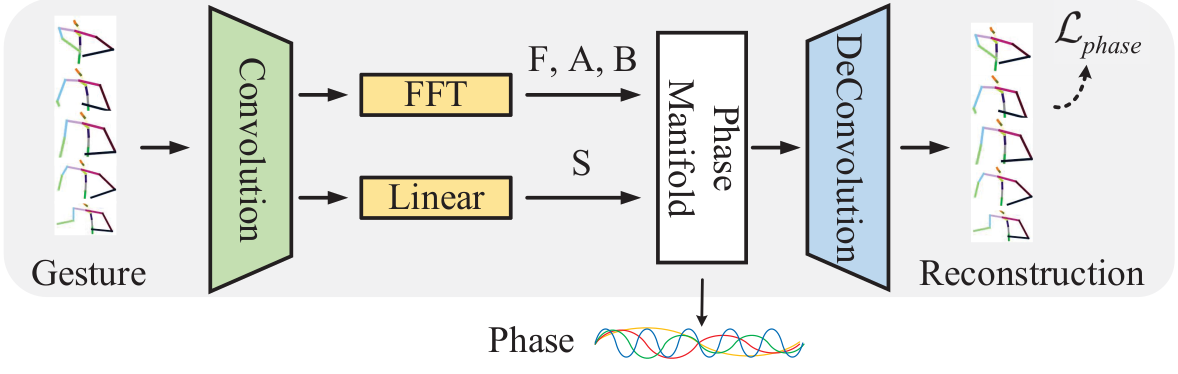
\includegraphics[width=\linewidth]{images/phrase_guidance.png}
%     \caption{Phrase Guidance}
%     \label{fig:PhraseGuidance}
% \end{figure}


% Hàm pha

% $$
% f(\mathcal{T} ; \mathbf{A}, \mathbf{F}, \mathbf{B}, \mathbf{S})=\mathbf{A} \cdot \sin (2 \pi \cdot(\mathbf{F} \cdot \mathcal{T}-\mathrm{S}))+\mathbf{B}
% $$

% Hàm encoder

% $$
% \mathbf{L}=E_{p}(\mathbf{G_{ \text{rotation\_velocity} }})
% $$

% Hàm fourier 
% $$
% \mathbf{c}=F F T(\mathbf{L});\ \ \mathbf{c} \in \mathbb{C}^{M \times K+1}, K=\left|\frac{T}{2}\right|
% $$

% $$
% \mathbf{f}=(0,1 / N, 2 / N, \ldots, K / N)
% $$

% $$
% \mathbf{A}_{i}=\sqrt{\frac{2}{T} \sum_{j=1}^{K} \mathbf{p}_{i, j}}
% $$

% $$
% \quad \mathbf{F}_{i}=\frac{\sum_{j=1}^{K}\left(\mathbf{f}_{j} \cdot \mathbf{p}_{i, j}\right)}{\sum_{j=1}^{K} \mathbf{p}_{i, j}}
% $$


% $$
% \quad \mathbf{B}_{i}=\frac{\mathbf{c}_{i, 0}}{T},
% $$

% Phrase shift
% $$
% \left(s_{x}, s_{y}\right)=F C\left(\mathbf{L}_{i}\right), \quad \mathbf{S}_{i}=\operatorname{atan} 2\left(s_{y}, s_{x}\right)
% $$

% $$
% \mathcal{T}=\left[-\frac{t_{1}-t_{0}}{2},-\frac{t_{1}-t_{0}}{2}+\frac{t_{1}-t_{0}}{N-1}, \ldots, \frac{t_{1}-t_{0}}{2}\right]
% $$


% $$
% \hat{\mathbf{L}}=f(\mathcal{T} ; \mathbf{A}, \mathbf{F}, \mathbf{B}, \mathbf{S})=\mathbf{A} \cdot \sin (2 \pi \cdot(\mathbf{F} \cdot \mathcal{T}-\mathrm{S}))+\mathbf{B}
% $$

% $$
% \hat{\mathbf{G}}_{2}=h(\hat{\mathbf{L}})
% $$

% $$
% \mathcal{P}_{2 i-1}^{(t)}=\mathrm{A}_{i}^{(t)} \cdot \sin \left(2 \pi \cdot \mathrm{S}_{i}^{(t)}\right), \mathcal{P}_{2 i}^{(t)}=\mathrm{A}_{i}^{(t)} \cdot \cos \left(2 \pi \cdot \mathrm{S}_{i}^{(t)}\right)
% $$

% $$
% \mathcal{P} \in \mathbb{R}^{2\ M}
% $$

% $$\mathcal{L}_{\text {phase }}=\mathcal{L}_{\text {phase-recon }}\left(\mathbf{G}, \hat{\mathbf{G}}_{\mathbf{2}}\right)$$




% $$
% \left(
% \left[
%     \hat{
%     \mathcal{P}}_o[-1]^{
%     \left[
%     \left(N_{
%     \text{strid}}-N_{
%     \text{phase}}
% \right):
% \right]}, 
% \mathcal{P}_{a, t}^{
%     \left[N_{
%     \text{strid}}:
% \right]}
% \right]
% \right. 
% , 
% \left.
% \left[
%     \hat{
%     \mathcal{P}}_o[-1]^{
%     \left[-N_{
%     \text{strid}}:
% \right]}, 
% \mathcal{P}_{a, t}^{
%     \left[
%     \left(N_{
%     \text{phase}}-N_{
%     \text{strid}}
% \right):
% \right]}
% \right]
% \right)<
% $$


% $$
% \left(\left[    \hat{    \mathcal{P}}_o[-1]\left[    \left(N_{    \text{strid}}-N_{    \text{phase }}\right):\right], \mathcal{P}_{t, t}^{    \left[        N_{    \text{strid}}:\right]}\right]\right. ,    \left.\left[    \hat{    \mathcal{P}}_o[-1]^{    \left[        -N_{    \text{strid}}:\right]}, \mathcal{P}_{t, t}^{    \left[    \left(N_{    \text{phase }}-N_{    \text{strid}}\right):\right]}\right]\right)
% $$



% $$
% d\left(\operatorname{concat}\left[\hat{\mathcal{P}}_o[-1]\left[\left(N_{\text {strid }}-N_{\text {phase }}\right):\right], \mathcal{P}_{t, t}^{\left[N_{\text {strid }}:\right]}\right]\right. \text {, }   \left.\operatorname{concat}\left[\hat{\mathcal{P}}_o[-1]^{\left[-N_{\text {strid }}:\right]}, \mathcal{P}_{t, t}^{\left[\left(N_{\text {phase }}-N_{\text {strid }}\right):\right]}\right]\right)
% $$

% $$
% d\left(\operatorname{concat}\left[\hat{\mathcal{P}}_o[-1]^{\left[\left(N_{\text {strid }}-N_{\text {phase }}\right):\right]}, \mathcal{P}_{a, t}^{\left[N_{\text {strid }}:\right]}\right]\right. \text {, }   \left.\operatorname{concat}\left[\hat{\mathcal{P}}_o[-1]^{\left[-N_{\text {strid }}:\right]}, \mathcal{P}_{a, t}^{\left[\left(N_{\text {phase }}-N_{\text {strid }}\right):\right]}\right]\right)<
% $$


% $$
% \left[\mathcal{P}_{-1}^{\left[\left(N_{\text {strid }}-N_{\text {phase }}\right):\right]}, \mathcal{P}_{a / t}^{\left[N_{\text {strid }}:\right]}\right]
% $$

% $
% \left[\mathcal{P}_{-1}^{\left[-N_{\text {strid }}:\right]}, \mathcal{P}_{a / t}^{\left[\left(N_{\text {phase }}-N_{\text {strid }}\right):\right]}\right]
% $
